\chapter{Determined protein structures}
\label{chapter:results}
This section describes all test-targets which I have attempted to fold using the methodologies presented in the previous chapters.
All protein structures, chemical shift and NOE data used in this thesis is available from \url{http://github.com/andersx/cs-proteins/}.


\section{Barley Chymotrypsin Inhibitor II}

An especially interesting target in this study is the barley chymotrypsin inhibitor II (CI-2). CI-2 is a 63 residue protein which consists of an $\alpha$-helix which connects via a very flexible handle to a small $\beta$-sheet region.

The chemical shifts data supplied by Kaare Theilum (personal communication) was obtained using a fully automated procedure.
The ADAPT-NMR \cite{adaptnmr} protocol was used to record all necessary NMR data and automatically assign the chemical shifts.
Data collection and assignment was completed in only 11 hours with minimal human intervention.
As we demonstrate, a structure could be determined computationally from these chemical shifts in only two days running on 12 cores.



\subsection{Computational methodology}
Several folding protocols were tried for this protein. All runs were performed as 72 independent trajectories which ran for 50 mio MC steps (iterations). Sampling was carried out using either TorusDBN or TorusDBN-CS to bias the backbone moves and the PROFASI force field was used in all simulations. Three simulations used an energy function based on CamShift using a cauchy distribution with variable $\gamma$ value as energy function. Additionally, three simulations used a potential on the radius of gyration to restrict the sampling to only compact structures. 
Sampling was performed in the multicanonical ensemble with a thermodynamic beta-range from 0.6 to 1.1, corresponding to a temperature range of 272K to 500K. The MC move set was comprised of 40\% CRISP moves, 10\% pivot moves and 50\% uniform side chain moves.


\begin{table}[h]
    \caption{Protocols used in the folding of the CI-2 protein and success rates.}
    \begin{center}
    \begin{threeparttable}
    \begin{tabular}{l l l l l l}
        Sampling        & Force Field   & CS Energy         & Correct fold\tnote{a} & Iterations/day\tnote{b}\\\hline
          TORUS-CS + PP\tnote{c} & PROFASI       & CamShift          & 13            & $10 \times 10^6$ \\
          TORUS-CS      & PROFASI       & CamShift          & 15            & $11 \times 10^6$\\
          TORUS         & PROFASI       & CamShift          & 0             & $11 \times 10^6$\\
 TORUS-CS + PP\tnote{c} & PROFASI       & None              & 4\tnote{d}      & $49 \times 10^6$\\
 TORUS-CS\tnote{e}+ PP\tnote{c} & PROFASI      & None              & 0             & $49 \times 10^6$\\
          TORUS-CS      & PROFASI       & None              & 0             & $49 \times 10^6$\\
          TORUS         & PROFASI       & None              & 0             & $49 \times 10^6$\\
    \end{tabular}
    \begin{tablenotes}
        \item[a] Number of threads with a CA-RMSD of $<5$ \AA\ (using all residues).\\
        \item[b] Numbers are \textit{per} thread.
        \item[c] PP denote the use of an additional radius of gyration potential\cite{Phaistos_oldest}.\\
        \item[d] Structures with the lowest energy did not correspond to the native structure in this run.\\
        \item[e] This run was carried out using TorusDBN-CS trained using only high-quality X-ray structures.
    \end{tablenotes}
    \end{threeparttable}
    \end{center}
    \label{tab:ci2}
\end{table}
\subsection{Folding results}
\label{sec:ci2_results}
Three of the 7 attempted simulation types sample structures close to the experimental X-ray structure 1YPA (here loosely defined as a CA-RMSD $<5$ \AA\ for all CA atoms. Results are summarized in table \ref{tab:ci2}.
Only simulations using chemical shift biased sampling through TorusDBN-CS are able to sample the correct fold.

Furthermore, it was noted, that simulations that sample from either TorusDBN or TorusDBN-CS with only the PROFASI force field as energy function do not generate compact structures.
To overcome this deficiency, additional simulations were carried out using a radius of gyration potential.
In the case of sampling from TorusDBN-CS, the radius of gyration potential is enough to get a few samples with the correct fold. Here four of 72 threads would generate the correct fold, but unfortunately the lowest energy structures were found around 8-11 \AA\ CA-RMSD. Evidently, the PROFASI force field alone is not accurate enough to describe the native CI-2 structure.
Three simulations were performed with an energy term based on CamShift in addition the PROFASI force field.
Demonstrably, the increased accuracy from a better energy function cause increased sampling around the native state.

Due to a very flexible region of CI-2 (residues 33 to 42), and somewhat flexible tails the residue range used to calculate CA-RMSD values is restricted to residue 4-34,43-63 in the following.
All runs were carried out on 3 24-core AMD Opteron 6172 servers running at 2.1 GHz. 

A run similar to the most successful was also run carried out on a faster a 12-core Intel X5675 node running at 3.07 GHz (using new random seeds).
PHAISTOS input to reproduce these folding simulation is given below.

\begin{lstlisting}
./phaistos --aa-file ci2.aa \
  --iterations 50000000 \
  --threads 12 \
  --monte-carlo-muninn 1 \
  --monte-carlo-muninn-min-beta 0.6 \
  --monte-carlo-muninn-max-beta 1.1 \
  --monte-carlo-muninn-independent-threads 1 \
  --monte-carlo-muninn-weight-scheme multicanonical \
  --backbone-dbn-torus-cs 1 \
  --backbone-dbn-torus-cs-initial-nmr-star-filename ci2.str \
  --energy-profasi-cached 1 \
  --energy-camshift-cached 1 \
  --energy-camshift-cached-star-filename ci2.str \
  --energy-camshift-cached-energy-type 11 \
  --move-backbone-dbn 1 \
  --move-backbone-dbn-weight 0.1 \
  --move-backbone-dbn-implicit-energy 1 \
  --move-crisp-dbn-eh 1 \
  --move-crisp-dbn-eh-weight 0.4 \
  --move-sidechain-uniform 1 \
  --move-sidechain-uniform-weight 0.5
\end{lstlisting}

This simulation took two days, with a total of 2 out of 12 threads successfully identifying the native structure as having the lowest energy.
This simulation yielded a lowest energy structure a 2.76 \AA~CA-RMSD from the X-ray structure, and a lowest RMSD structure at 1.11 \AA. Later, this lowest energy sample was further refined by Lars Bratholm to a CA-RMSD of only 1.1 \AA using an additional multibody-multinomial poteintial of mean force in the simulation\cite{mumu}, a procedure which took 24 hours on 8 cores.
In conclusion, the data for CI-2 was recorded in merely, 11 hours via fully automated process. A structure comparable to conventional NMR structures could then be determined after 36 hours. After an additional24 hours, a structure that rivals X-ray structures was further determined by Lars Bratholm.

\begin{figure}%
    \centering
    \subfloat[NMR structure (red)]{
        {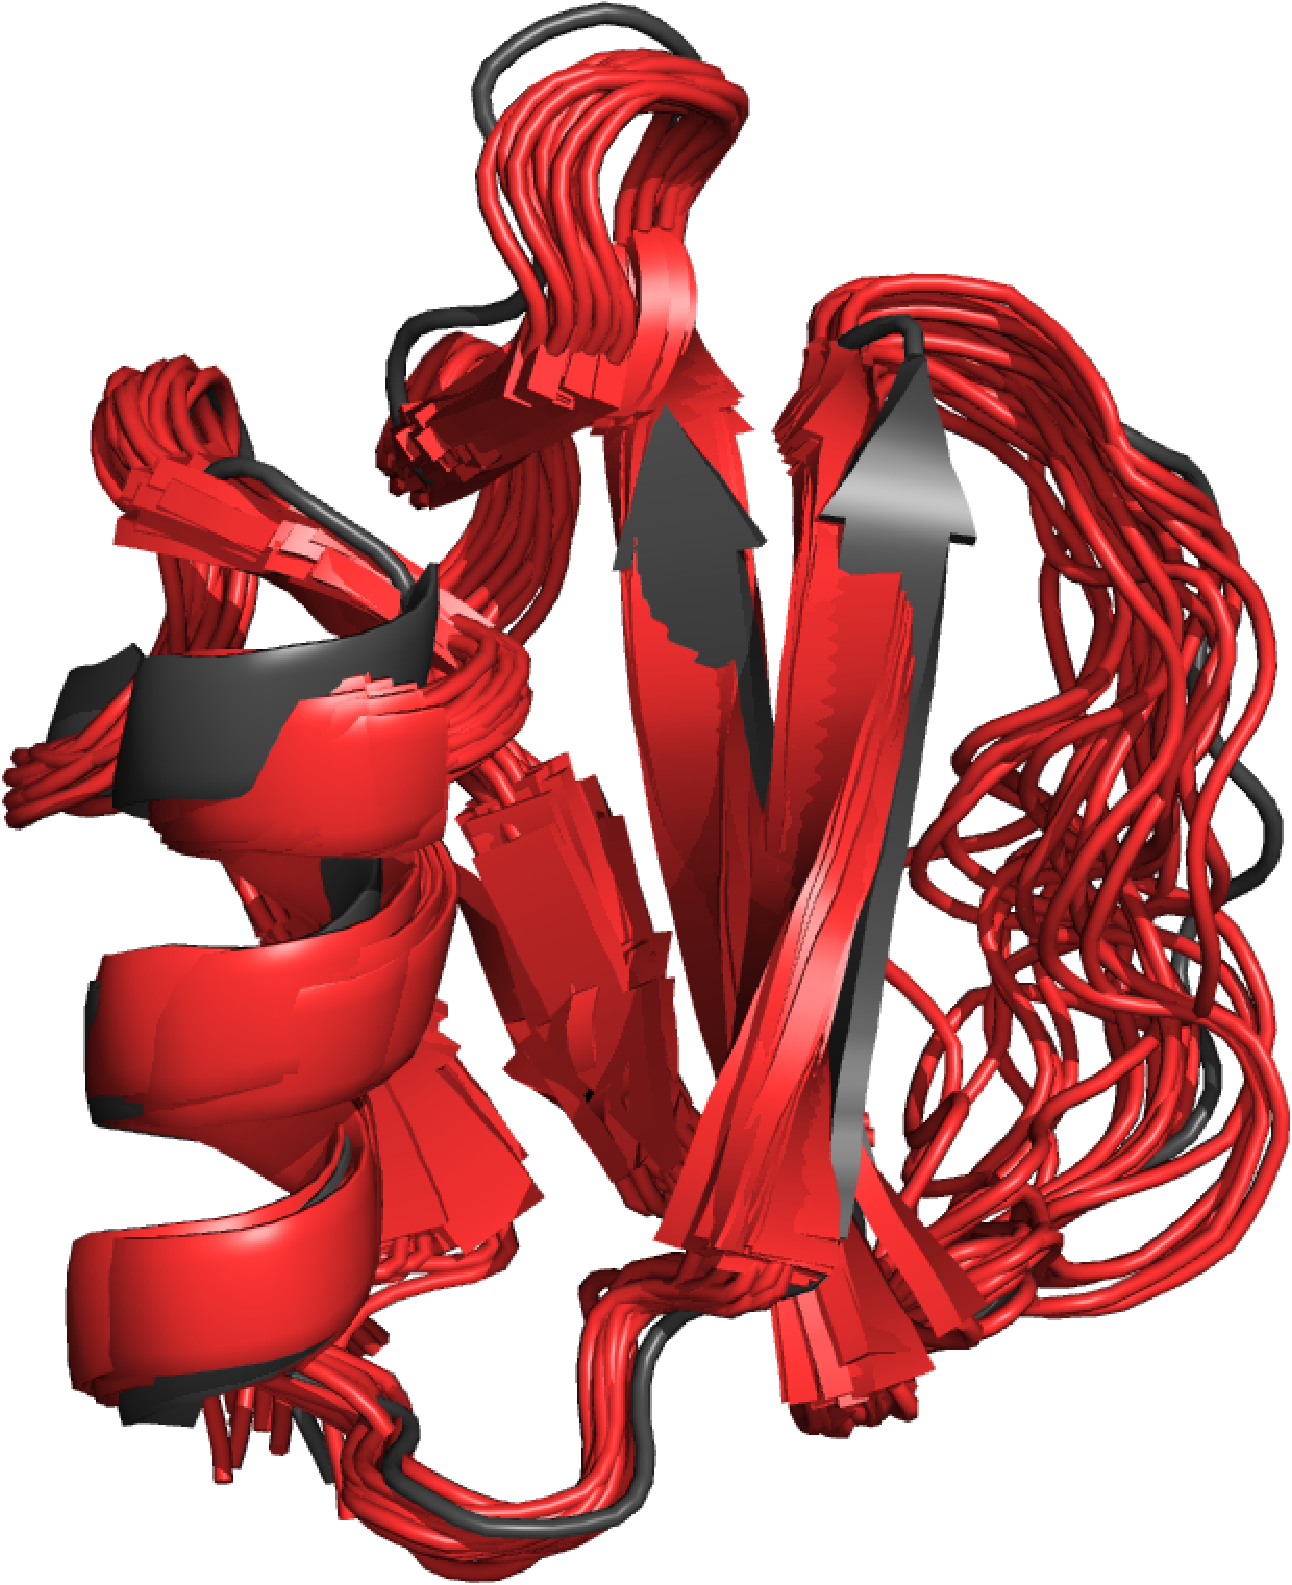
\includegraphics[width=0.3\textwidth]{figures/ci2_pymol/crystal_nmr_trim.pdf}}
    }
    \subfloat[Lowest RMSD structure (blue)]{
        {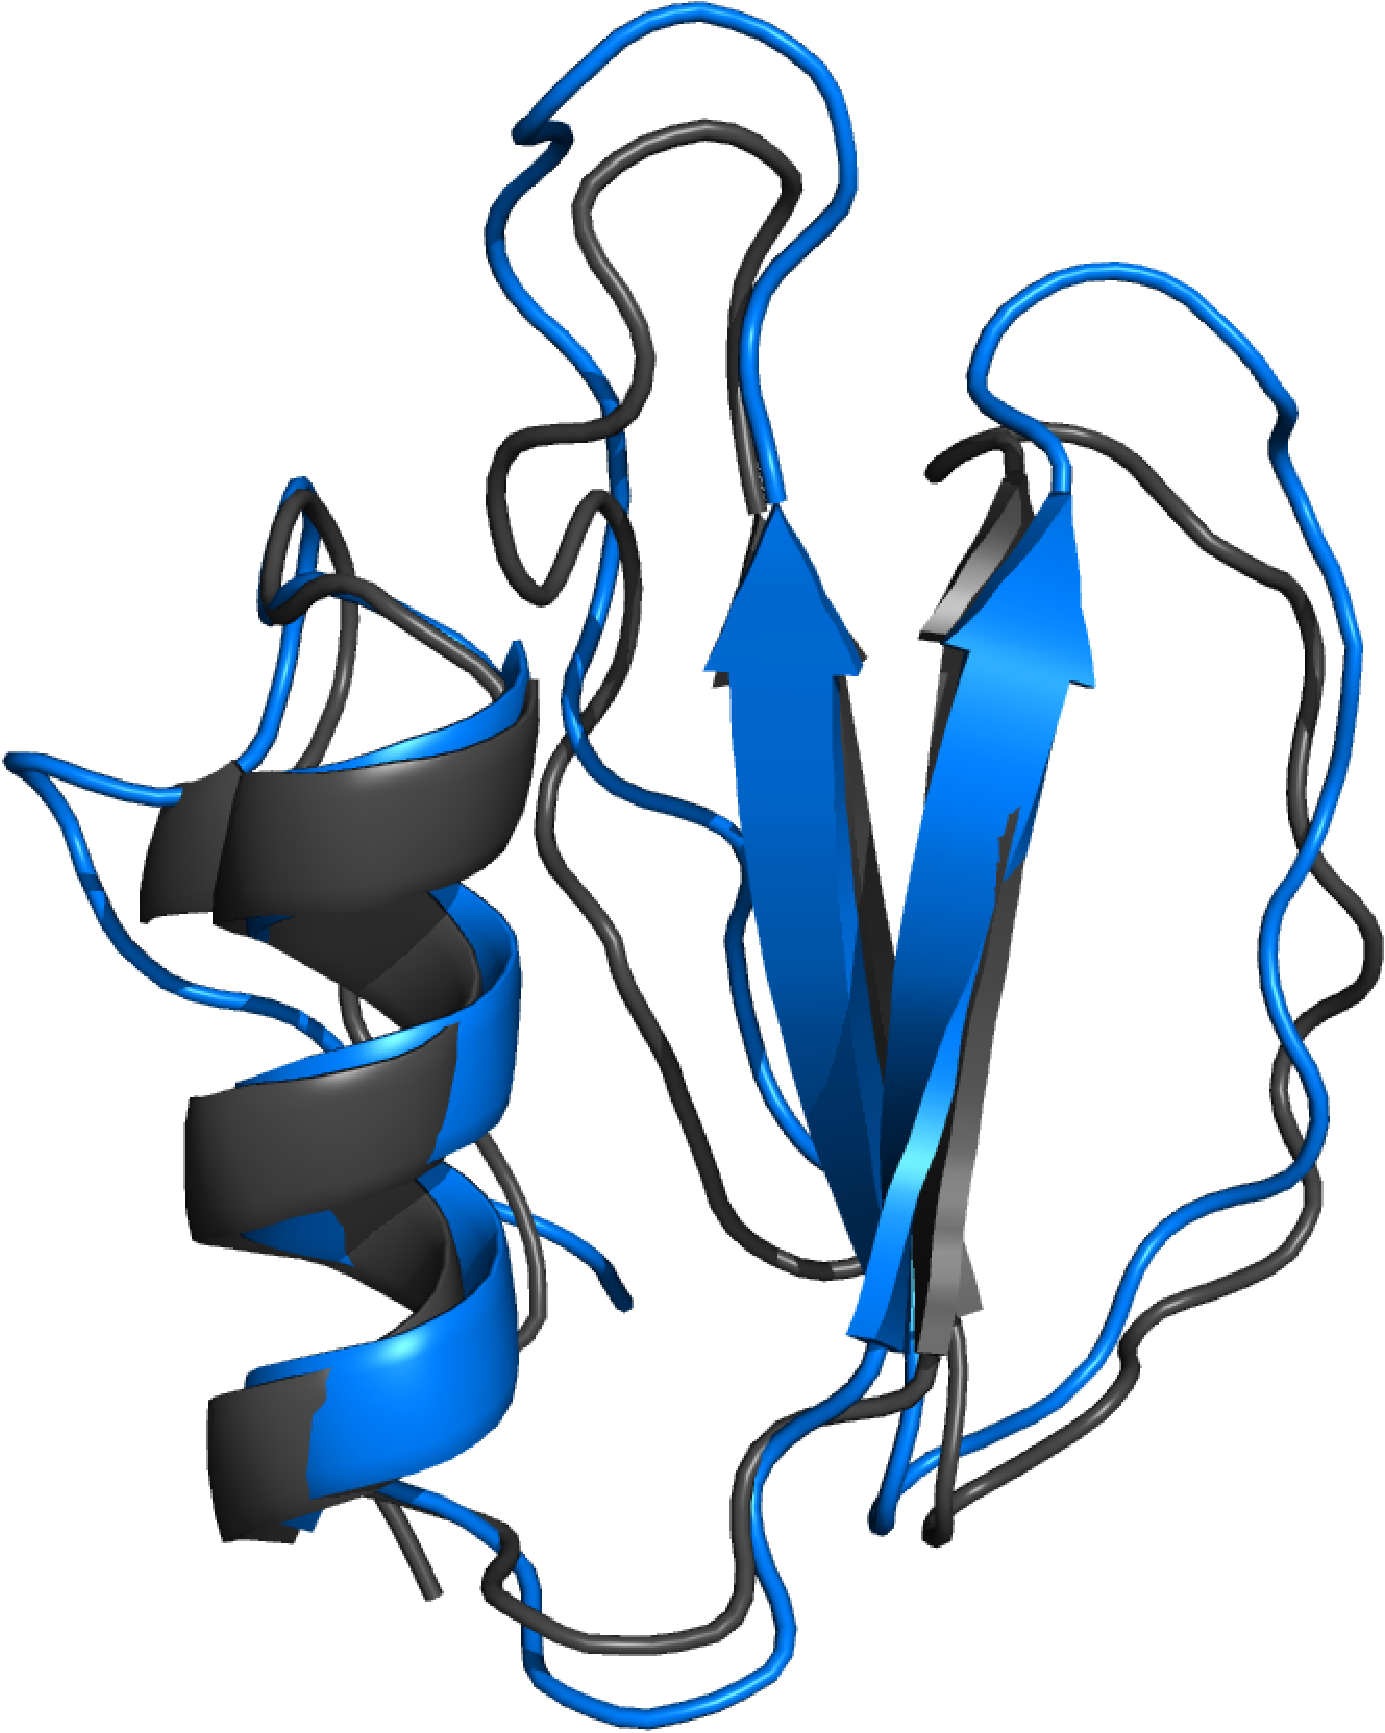
\includegraphics[width=0.3\textwidth]{figures/ci2_pymol/crystal_lowest_rmsd_trim.pdf}}
    }
    \subfloat[Lowest energy structure (green)]{
        {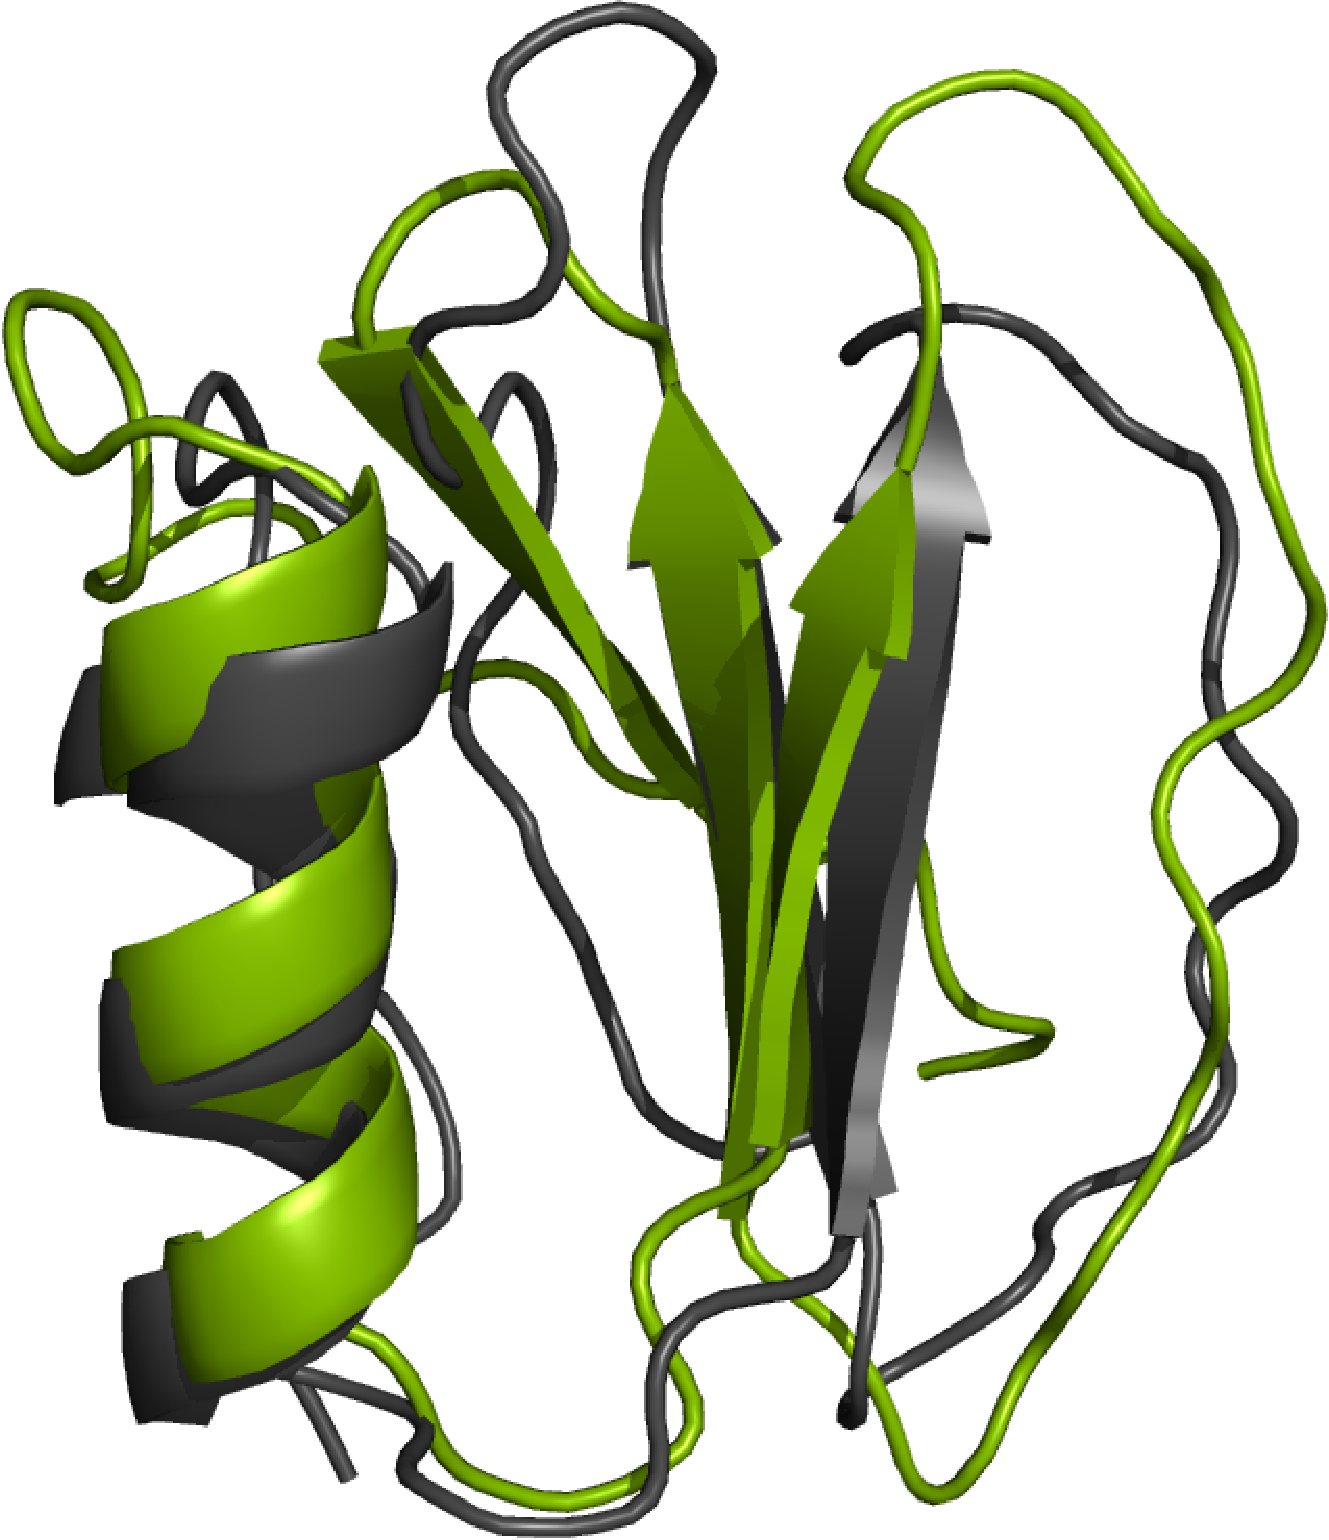
\includegraphics[width=0.3\textwidth]{figures/ci2_pymol/crystal_lowest_energy_trim.pdf}}
    }
    \caption{Structures compared to the X-ray structure 1YPA. All structures are aligned using the residues 12-32,43-52. (a) shows the 3CI2 structure NNR structure. Note the flexible domain which is excluded from the fit-range. (b) Shows the lowest RMSD structure (1.113 \AA RMSD). (c) shows the lowest energy sample (2.76 \AA RMSD). }
    \label{fig:ci2}%
\end{figure}



\section{Folding of small proteins (\textless 100 AA)}

A test set of 5 small proteins were folded using the code. The results are summarized in table \ref{tab:folding_small}. The test set is a diverse set of structures with different contents of alpha-helix and beta-sheet conformations. 
The settings are similar to the ones used to fold the CI-2 structure mentioned in the previous section, except that the Protein G, Ubiquitin, FF Domain and Engrailed Homeodomain (ENHD) simulations used a chemical shift energy based on a Gaussian distribution with fixed weights (--energy-camshift-cached-energy-type 3), and not based on a Cauchy distribution (--energy-camshift-cached-energy-type 11).
\begin{table}
    \caption{The five small proteins folded using the setup presented in this section, and their RMSD for the lowest energy sample.}
    \begin{center}
    \begin{threeparttable}
    \begin{tabular}{l l l l l  l l}
Name                & Lengh    & Type & PDB     & RefDB     & RMSD-range    & Final RMSD   \\\hline
Protein G           & 56       & a/b & 2OED    & 2575      & All           & 1.0           \\
% Can't find data for SMN Tudor Domain :( :( :( :( :(, only the 3.3 number :(
% SMN Tudor Domain    & 59       & a/b & 1MHN    & 4899      & 5-54          & 3.3       \\
Engrailed Homeodomain & 61     & B   & 1ENH    & 15536     & 8-53          & 1.1           \\
FF Domain           & 71       & a/b & 1UZC    & 5537      & 11-67         & 10.2         \\
Ubiquitin           & 76       & a/b & 1UBI    & 17769     & 1-70          & 3.8           \\
CI-2                & 63       & a/b & 1YPA    & N/A\tnote{a}& 4-34,43-63  & 2.6\tnote{b}
    \end{tabular}
    \begin{tablenotes}
    \item[a] Using automatically assigned data obtained from Kaare Theilum (personal communication - see \url{https://github.com/andersx/cs-proteins}).
    \item[b] The number reported is discussed in section \ref{sec:ci2_results}.
    \end{tablenotes}
    \end{threeparttable}
    \end{center}
    \label{tab:folding_small}
\end{table}
Total energy was calculated as the PROFASI force field energy plus the CamShift energy term based on a Gaussian distribution with fixed weights plus the likelihood from TorusDBN-CS.
Protein G and ENHD structures could be determined very reliably to CA-RMSDs of 1.0 \AA~and 1.1 \AA~from the experimental structures, respectively. The lowest energy structures are presented in Fig.~\ref{fig:small_pics}a and \ref{fig:small_pics}b.

For the FF Domain, a folded state with a lower energy than the native state was located.
A state corresponding to the correct fold was consistently being sampled in most threads, but the lowest energy stat was a misfold, where an alpha-helix towards the C'-end is packed wrongly.
This result suggests, that the combination of the PROFASI force field and the chemical shift energy from CamShift and TorusDBN-CS does not always discriminate the potential energy surface with sufficient accuray. The energy from CamShift (and thus the chemical shift RMSD values, since the energy function was a Gaussian distribution) was comparable between samples around the correct fold and the lowest energy mis fold. The lowest RMSD structre (3.2 \AA) had a CamShift energy of 803 kcal/mol, while the lowest energy structure had a CamShift energy of 797 kcal/mol.
The lowest energy misfold is displayed in Fig.~\ref{fig:small_pics}c.
In the Ubiquitin simulations, the lowest energy conformations were not in exceptional agreement with the experimental structure with a CA-RMSD of 3.8 \AA - see Fig.~\ref{fig:small_pics}d.
 Again, this must be attributed to lack of "funneling" of the energy landscape around the native state, since sampling evidently is performed close to this state.

Collectively, these result show, that sampling from TorusDBN-CS in PHAISTOS is indeed very efficient, but better energy functions are required in some cases. In one case, the CamShift energy term had a lower energy by 6 kcal/mol for a misfold, than for a sample close to the native state.
Another option would be using a better molecular mechanics force-field. PHAISTOS already supports the OPLS-AA/L but this would increase simulation times by more than one order of magnitude, and would be unacceptable for simulations on larger structures.

\begin{figure}
    \centering
    \subfloat[Protein G, 1.0 \AA.]{
        {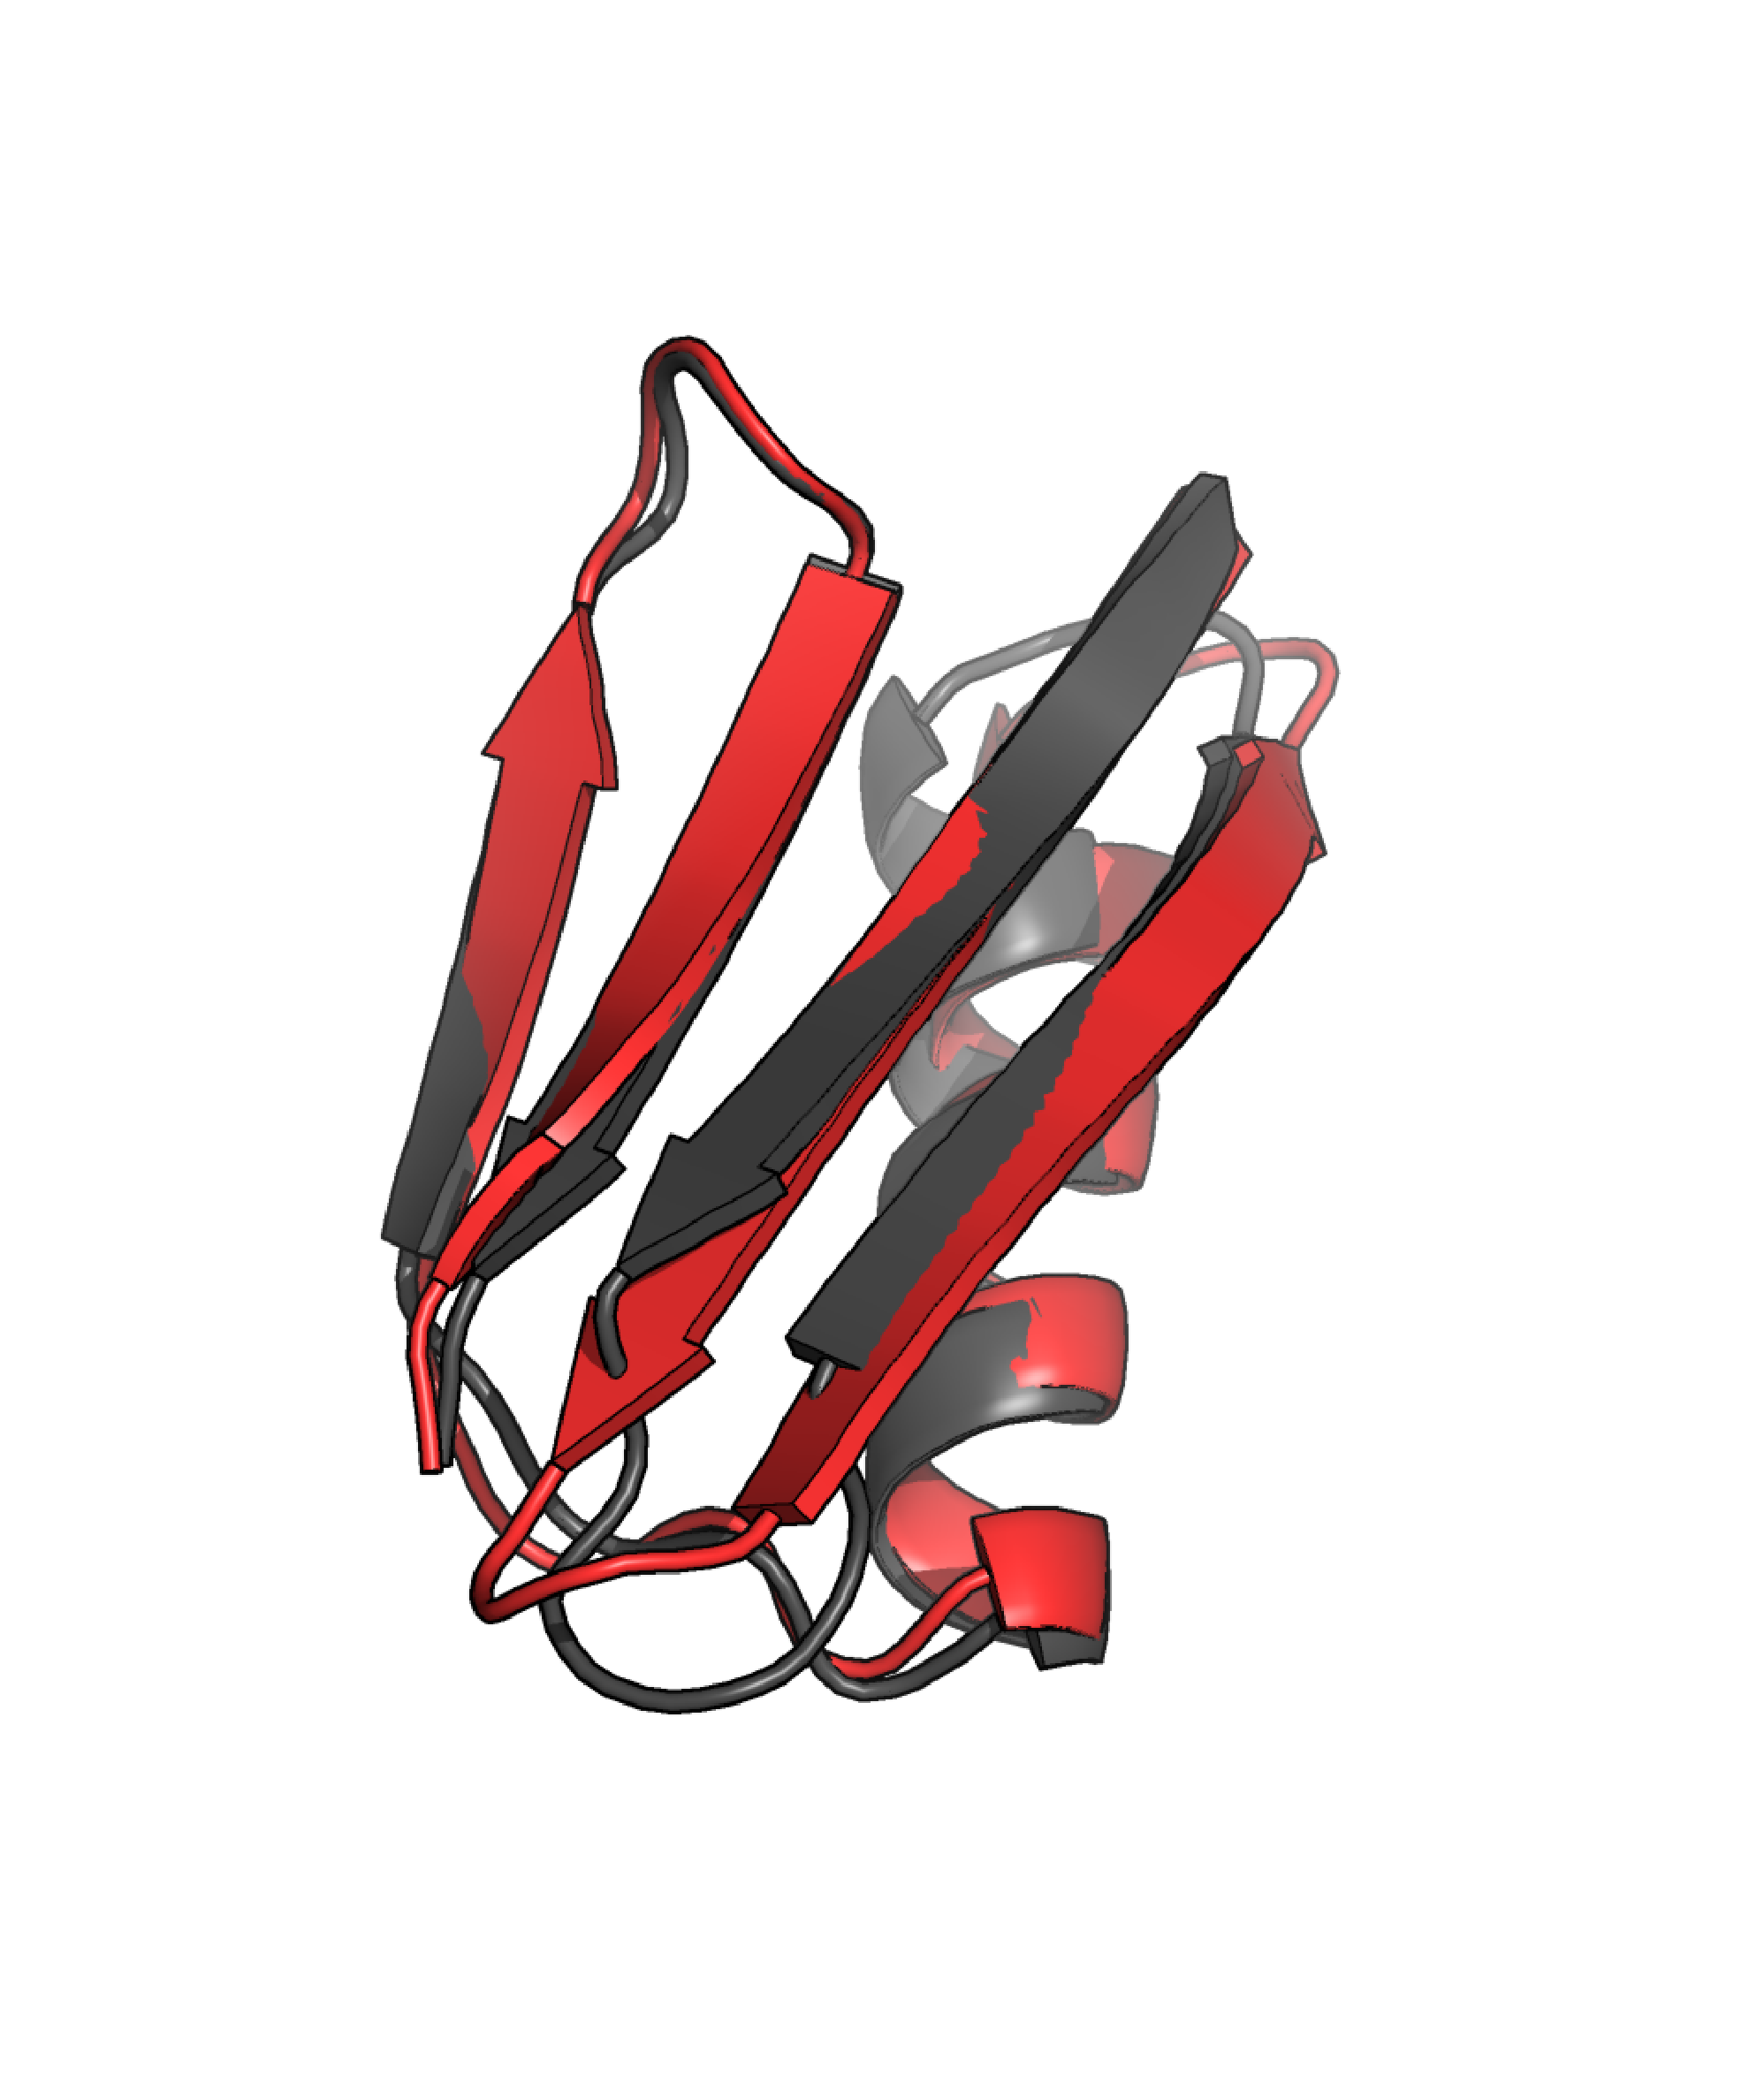
\includegraphics[width=0.45\textwidth]{figures/small_proteins/protein_g_min_e.pdf}}
    }\quad
    \subfloat[Engrailed Homeodomain, 1.1 \AA.]{
        {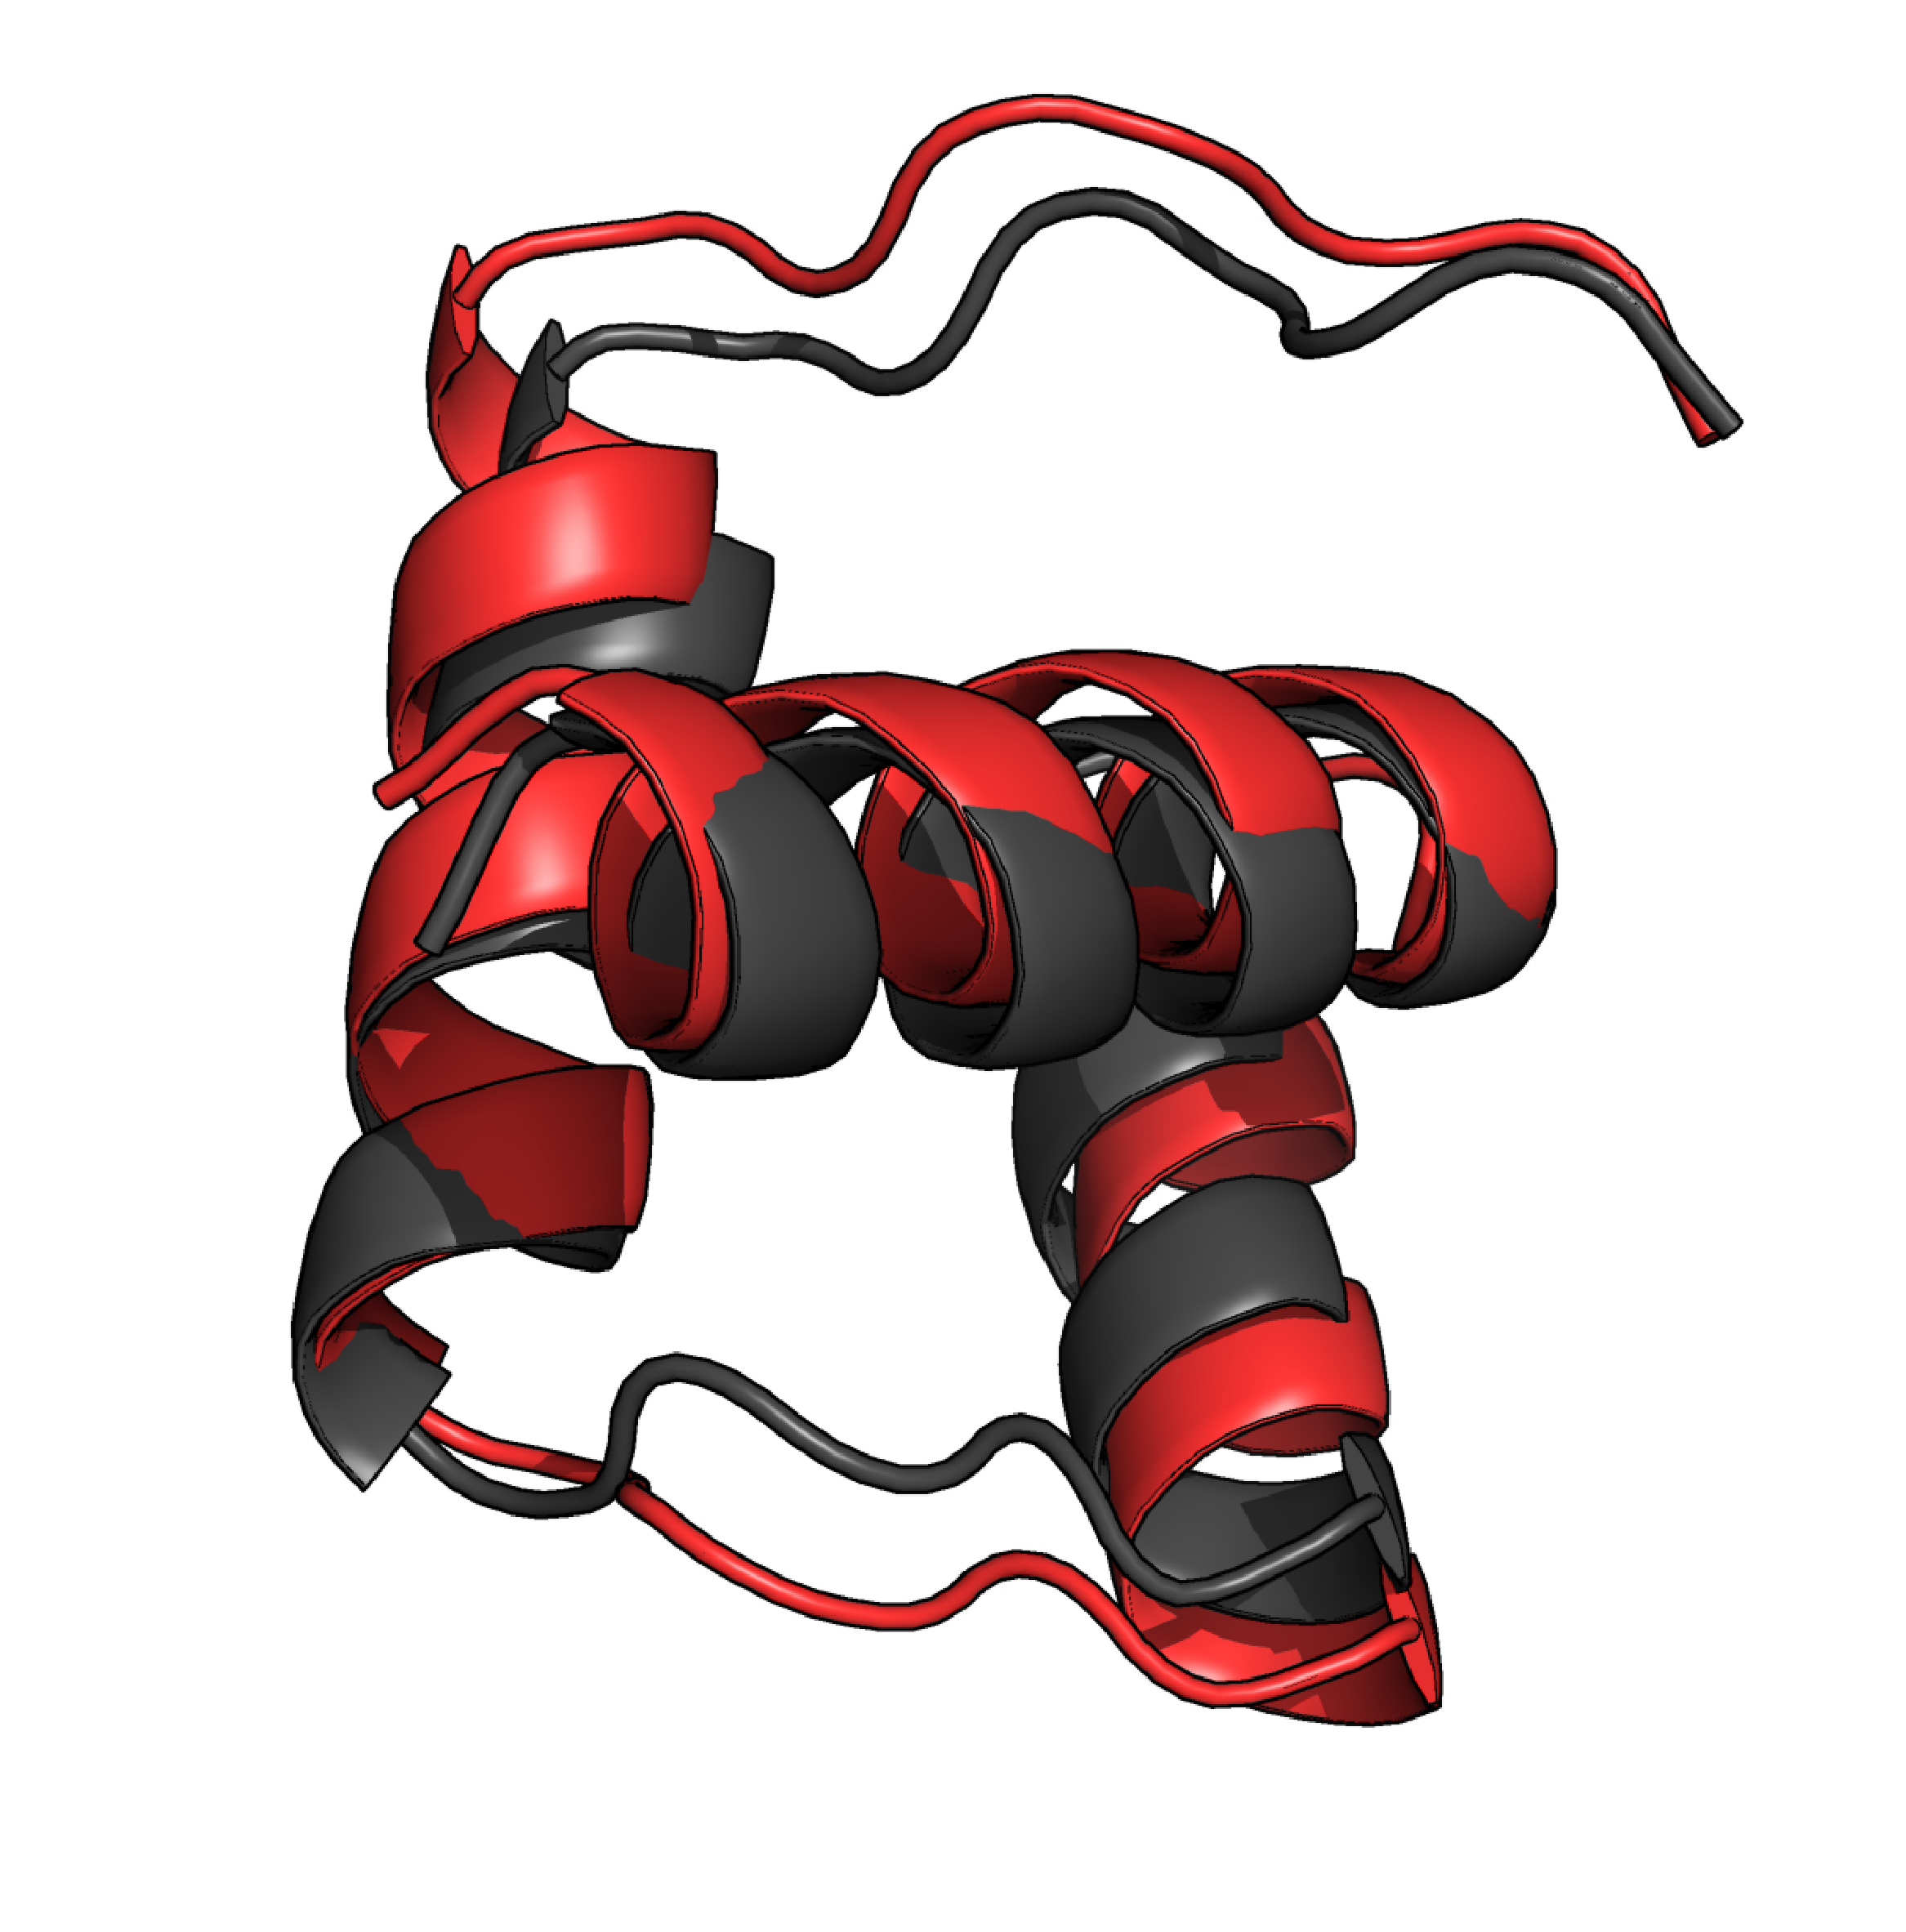
\includegraphics[width=0.45\textwidth]{figures/small_proteins/enhd_min_e.pdf}}
    }\\
    \subfloat[FF Domain, misfold.]{
        {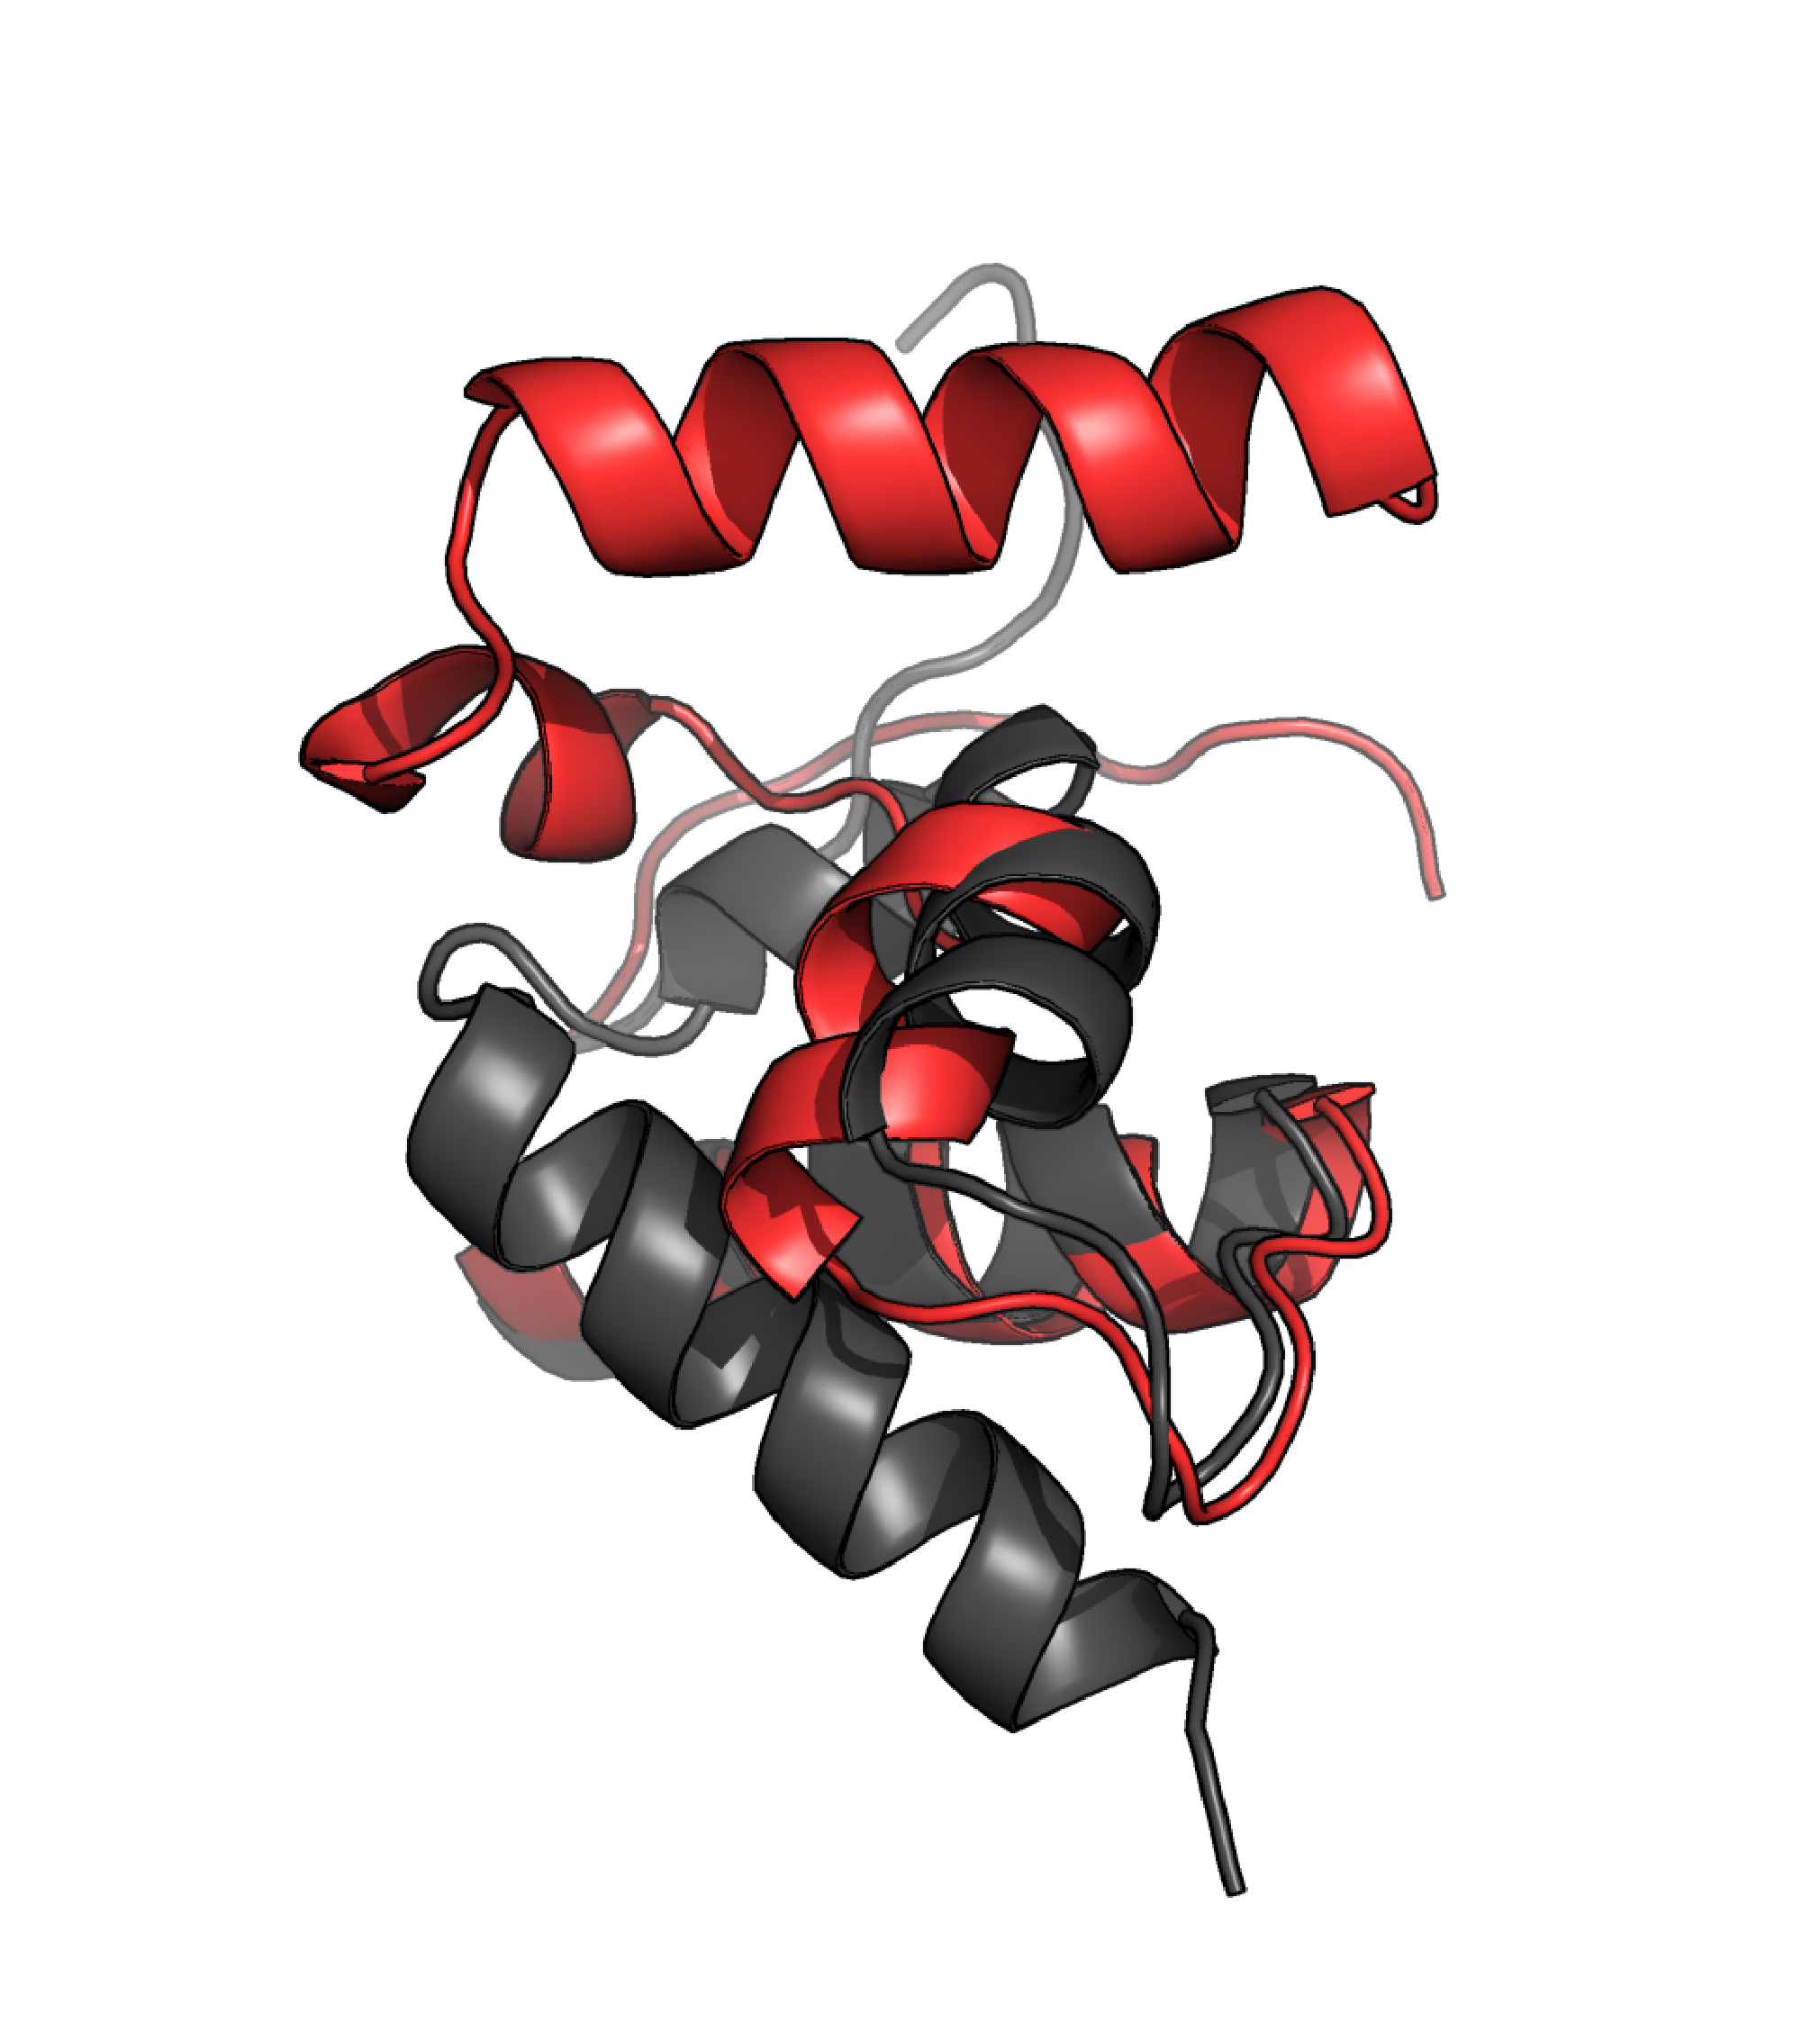
\includegraphics[width=0.45\textwidth]{figures/small_proteins/ff_domain_min_e.pdf}}
    }\quad
    \subfloat[Ubiquitin, 3.8 \AA]{
        {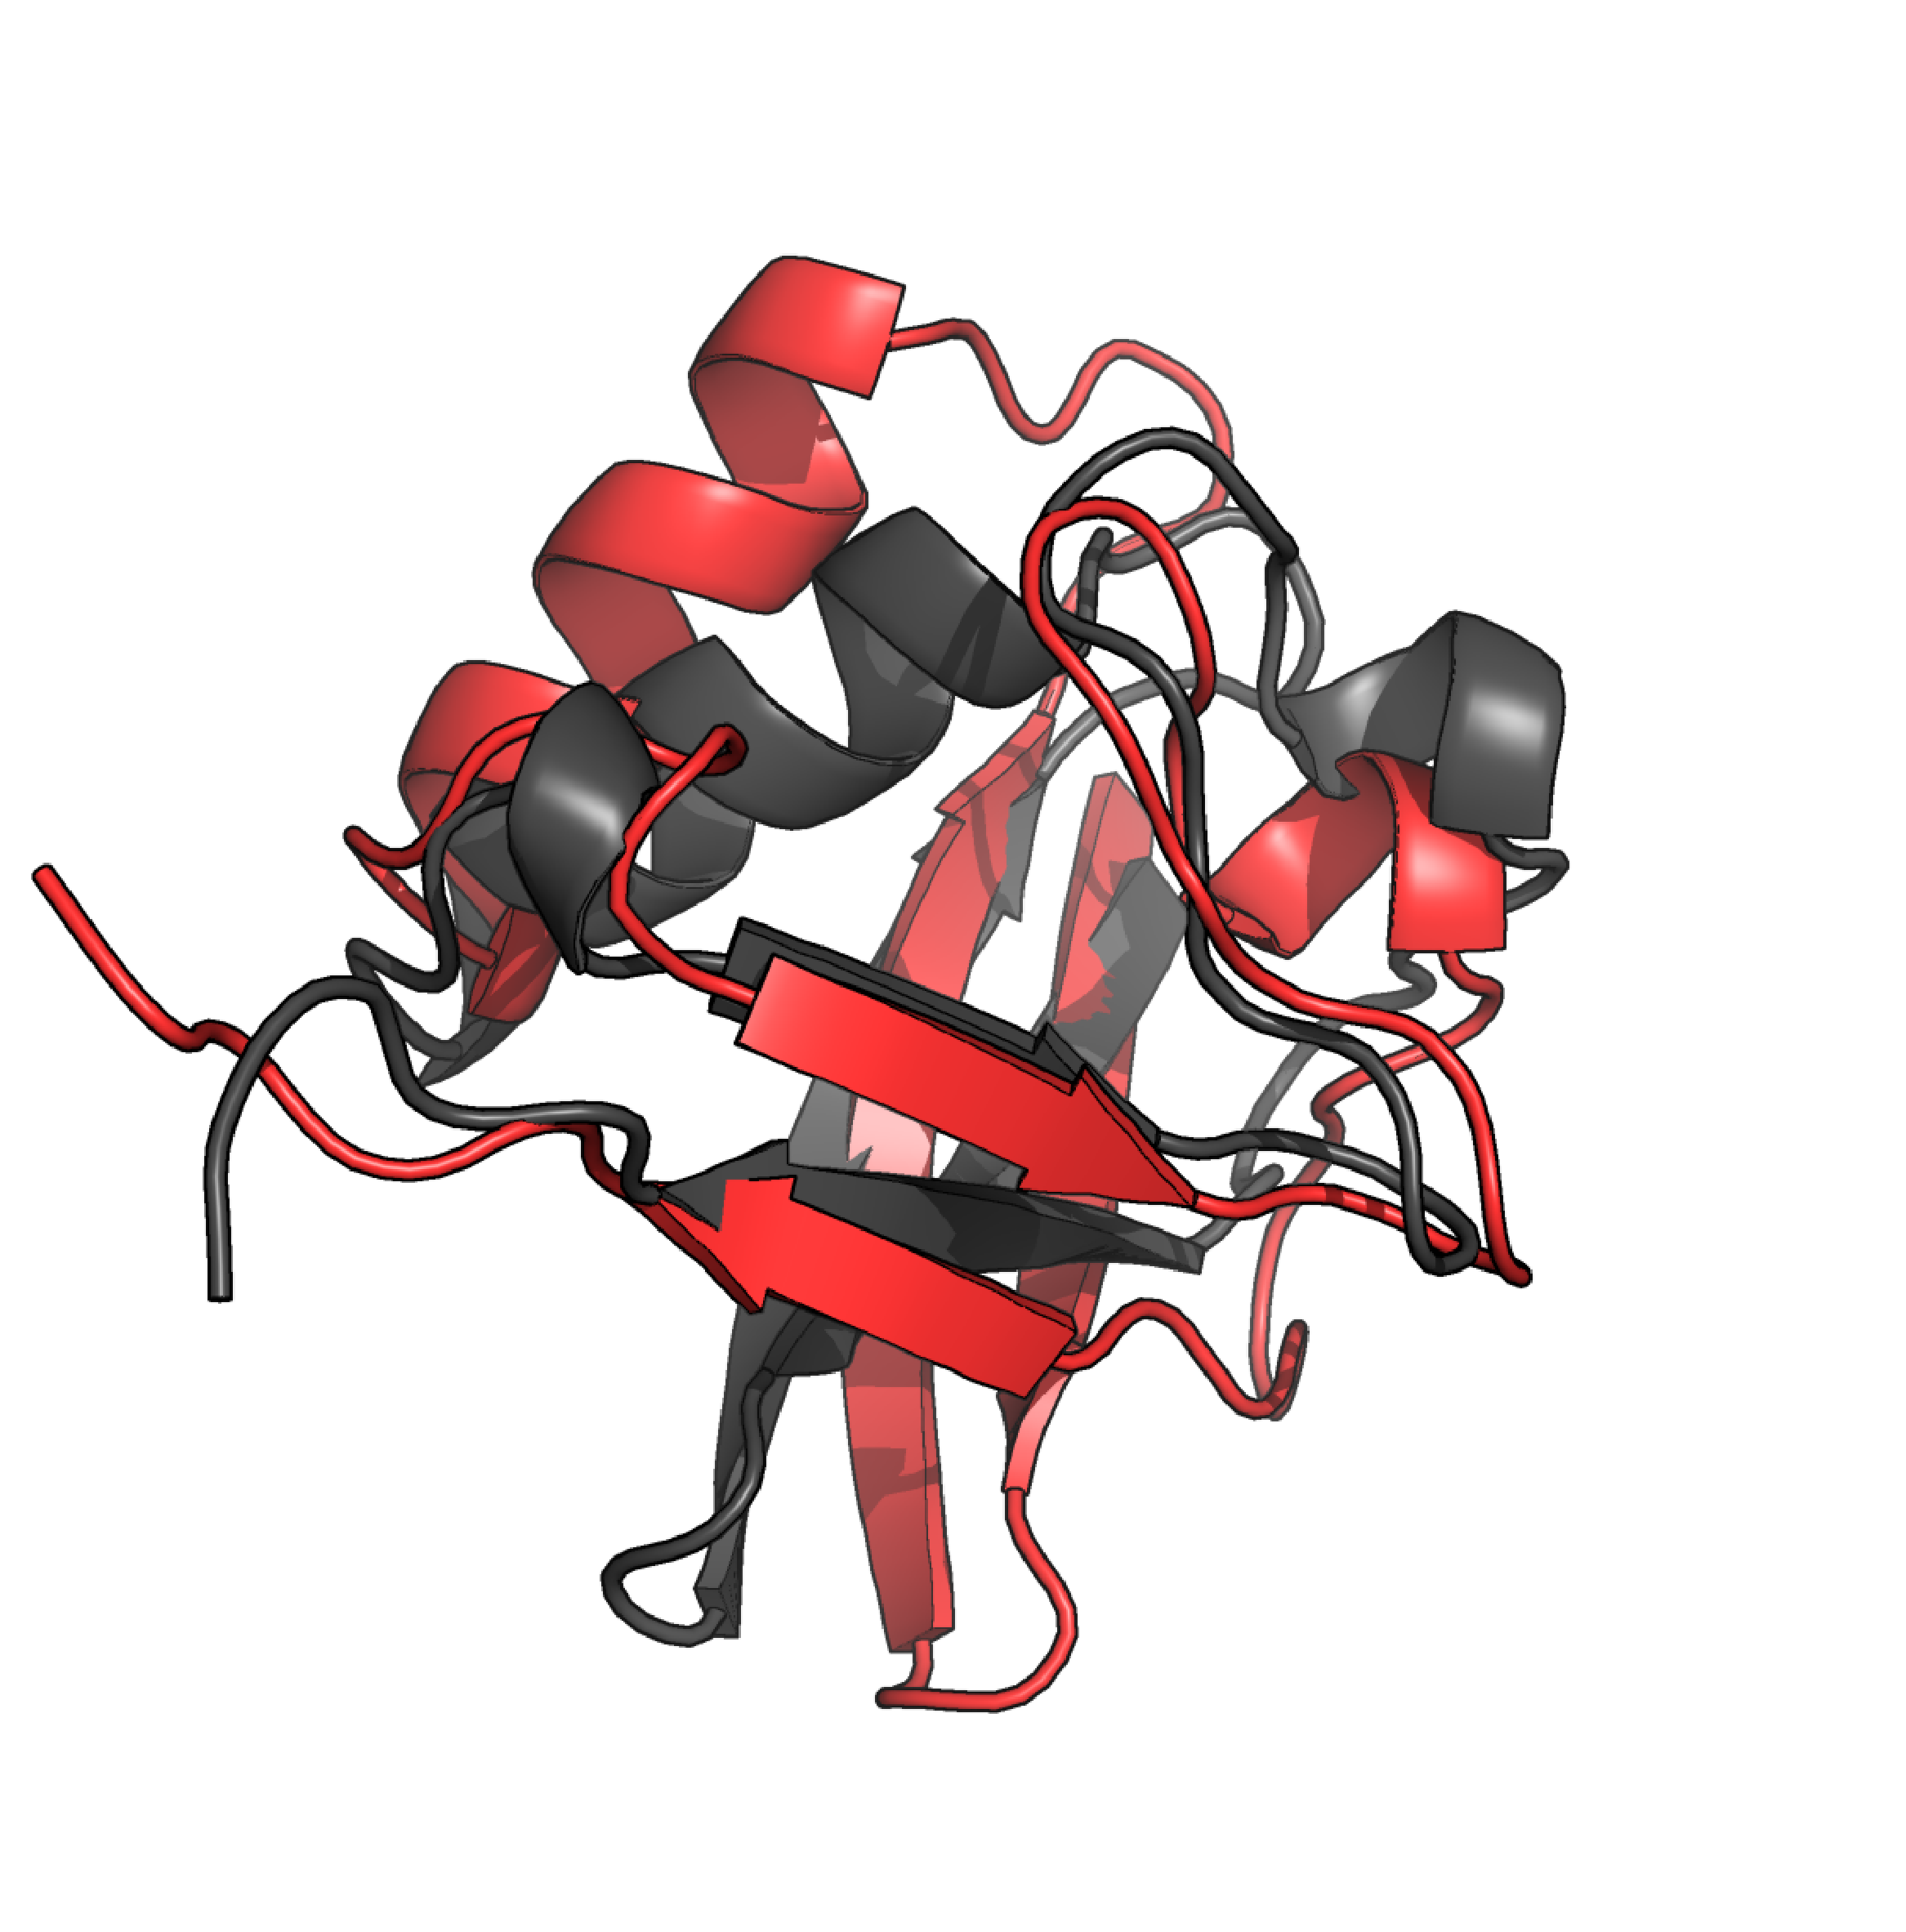
\includegraphics[width=0.45\textwidth]{figures/small_proteins/ubiquitin_min_e.pdf}}
    }\\
    \caption{The lowest energy structures found for four different proteins (red). Superimposed on corresponding X-ray structures (grey). The FF Domain structures in (c) is aligned using only residues 1-40 to emphasize the misfold.}
    \label{fig:small_pics}%
\end{figure}



\clearpage

\section{Folding of larger proteins (\textgreater 100 AA)}

This section presents folding results on a set of larger proteins (\textgreater 100 AA) with known structures.
It is worth to note, that using sparse NMR data, only three structures \textgreater 200 residues have been determined: Alg13 (201 AA), Rhodopsin (225 AA) and MBP (376 AA) using the ROSETTA program with the "resolution-adapted structural recombination" (RASREC) protocol\cite{Lange2012,LangePNAS2012}.

Alg13 was solved using backbone chemical shifts, and only 52 NOE restraints, to an CA-RMSD of 4 \AA~to the experimental NMR structure (2jzc).
Rhodopsin was folded to an CA-RMSD of 1.9 \AA~to the X-ray structure using 215 NOE restraints, backbone chemical shifts chemical shifts and RDCs.
The MBP protein is a two-domain protein of 376 residues.
MBP was folded to an RMSD of 3.6 \AA~using 1235 NOE restraints, backbone chemical shifts chemical shifts and RDCs.
The NOEs corresponded to 55\% yield of restraints, which, for the most part,  were not automatically assigned.
An attempt to use only automatically assigned NOEs yielded 455 restraints, which corresponds to a yield of 20\%. Using these, however, the MBP structure could only be determined to a total CA-RMSD of 12.3 \AA.
The N-terminal domain was converged to 2.7 \AA, but the C-terminal domain and the angle between the two domains was incorrectly folded.

Langer \textit{et al.} have demonstrated that by using a special side-chain labeling scheme a few NOE restraints (around 150-250) can be automatically assigned, and these are generally enough to fold the structures using a ROSETTA protocol\cite{LangePNAS2012}.
The scheme is a "ILV-labeling" scheme, where the methyl groups of isoleucine, leucine and valine side-chains are selectively labeled with $^{13}$C and $^1$H isotopes. These groups are commonly found in the core region of the protein and these methyl groups will generally be in contact with each other, thus being able to provide valuable NOE distance restraints.

From the structures in the study by Langer \textit{et al.}, only five structures consist of one chain only, and only those could be simulated in PHAISTOS.
These five structures were selected into the test-set used here, and additionally Prolactin and the Top7 proteins were added.
The ILV-data used by Langer \textit{et al.} could only be obtained through correspondence with the authors for Rhodopsin. 
For all other proteins, synthetic NOE contacts were generate by simulating a synthetic spectrum.
An overview of the proteins and the number of synthetic NOE restraints can be found in Table \ref{tab:folding_large}.




\begin{table}[h]
    \caption{Folded structure.}
    \begin{center}
    \begin{threeparttable}
    \begin{tabular}{l l l l r l r l}
Name                & Lengh    & Type   & PDB     & BMRB    & RMSD-range    & \#NOEs &  RMSD  [\AA]\\\hline
%APO-LFABP           & 129      & a/b    & 1LFO    & 15429\tnote{a}  & All  &      &   \\
Top7                & 120      & a/b    & 2MBL    & 19404     & 5-104       &  62   & 2.1 \\
MSRB                & 151      & a/b    & 3E0O    & 17008     & 36-105      & 170   & N/A \\
WR73                & 183      & a/b    & 2LOY    & 16833     & 1-36,66-181 & 215   & N/A \\
HR4660B             & 174      & a/b    & 2LMD    & 1870      & 16-162      & 68    & N/A \\
Rhodopsin           & 219      & B      & 2KSY    & 16678     & All         & 195   & 2.5 \\
Prolactin           & 199      & B      & 1RWS    & 5599      & 6-183       & 68    & 3.5 \\
Savinase            & 269      & a/b    & 1WVN    & Note\tnote{a,b} & Note\tnote{b} & 270 & 2.9 \\
MBP                 & 376      & a/b    & 1EZ9    & 6807      & All         &  1054 & N/A
    \end{tabular}
    \begin{tablenotes}
    \item[a] Evolutionary distance constraints from the EVFold were used in this case.
    \item[b] Available from: \url{http://github.com/andersx/cs-proteins/}
    \end{tablenotes}
    \end{threeparttable}
    \end{center}
    \label{tab:folding_large}
\end{table}

\subsection{Folding protocol}


The folding simulation settings were similar to those used to fold small proteins, with the exception that the CamShift energy term was too slow to be used in practice.
The additional NOE distance restraint term used a flat-bottom potential with a width of 4 \AA around the equilibrium distance, and a quadratic potential outside this range.
This was done using the existing NMR inference module in PHAISTOS.

However, using this potential turned out to be quite problematic. 
Once a distance restraint was fulfilled, the simulation would in most cases never break the contact again.
Consequently, an empirical factor of 1/128 was multiplied onto the NOE energy.
This factor was determined by running simulations on the Top7 structure with weights from $2^1$ to $2^{10}$
Unfortunatly, due to this problem, no good structures for MSRB, WR73, HR4660B and MBP could be located. 
After a few 1,000,000 steps the structures located local minima which fulfilled a number of distance restraints, but it was impossible to escape these minima.
The Top7 structure folded to an RMSD of 2.1 \AA.
This result, however, is not surprising, since Top7 has been shown to fold using only the PROFASI force field.
The Prolactin and Rhodopsin structures converged to structures at 8.5 and 7.8 \AA~RMSD from the X-ray structures.
\\\\The settings to run the simulations are displayed below:
\begin{lstlisting}
./phaistos --aa-file rhodopsin.aa \
  --iterations 50000000 \
  --threads 72 \
  --monte-carlo-muninn 1 \
  --monte-carlo-muninn-min-beta 0.6 \
  --monte-carlo-muninn-max-beta 1.1 \
  --monte-carlo-muninn-independent-threads 1 \
  --monte-carlo-muninn-weight-scheme multicanonical \
  --backbone-dbn-torus-cs 1 \
  --backbone-dbn-torus-cs-initial-nmr-star-filename \
                                      rhodopsin.str \
  --energy-profasi-cached 1 \
  --energy-isd-dist 1 \
  --energy-isd-dist-likelihood square_well \
  --energy-isd-dist-data-filename noe_ilv.txt \
  --energy-isd-dist-sample-gamme 0 \
  --energy-isd-dist-sample-sigma 0 \
  --energy-isd-dist-weight 0.0078125 \
  --move-backbone-dbn 1 \
  --move-backbone-dbn-weight 0.08 \
  --move-backbone-dbn-implicit-energy 1 \
  --move-crisp-dbn-eh 1 \
  --move-crisp-dbn-eh-weight 0.42 \
  --move-sidechain-uniform 1 \
  --move-sidechain-uniform-weight 0.5
\end{lstlisting}

\subsection{Refinement protocol}

Due to the low efficiency of the NOE code for large structures, a new NOE module was written for PHAISTOS. In this module, the potential from the ROSETTA RASREC protocol was used \cite{LangePNAS2012}.
In brief, this is also a flat-bottom potential, but with a linear penalty, rather than quadratic, outside the flat area.
This was done in order to allow more contacts to be broken throughout the simulation in order to enhance conformational sampling.
Additionally, the module only has a certain fraction of all restraints active at a time.
A Monte Carlo move was created which turned off one random, active NOE restraint and activated one random, deactivated restraint.
The resulting energy difference was subtracted as a move-bias, in order to force a 100\% acceptance rate for this move.
This was done, because the energy difference between and active restraint (which is usually close to zero) and an inactive restraint (usually a large number) caused this move to have a low acceptance rate.

Using the new NOE module, a refinement on the lowest energy structures in the Prolactin and Rhodopsin simulations were carried out.

The new module proved very efficient in further minimizing the energy.
Fig.~\ref{fig:rhodopsin} shows the resulting structures and energy/RMSD landscapes from the refinements and folding simulations on Rhodopsin.
The final RMSD after refinement was 2.5 \AA~for Rhodopsin, compared to 7.8 \AA~before refinement.
For Prolactin, the same numbers were 3.5 \AA~and 8.5 \AA, respectively.
The reason for the higher RMSD for Prolactin, compared to Rhodopsin is a flexible handle with no NOE restraints.
The structure of this handle is thus determined by the PROFASI force field and TorusDBN-CS, which apparently does not agree well with the experimental structure in this case - this can be seen from Fig.~\ref{fig:rhodopsin}.
\\\\The command line to run the refinement is given below:
\begin{lstlisting}
./phaistos --pdb-file rhodopsin_lowest_energy1.pdb \
  --init-from-pdb 1 \
  --iterations 5000000 \
  --threads 4 \
  --monte-carlo-muninn 1 \
  --monte-carlo-muninn-min-beta 0.6 \
  --monte-carlo-muninn-max-beta 1.1 \
  --monte-carlo-muninn-independent-threads 1 \
  --monte-carlo-muninn-weight-scheme multicanonical \
  --monte-carlo-muninn-weight-scheme-use-energy2 1 \
  --backbone-dbn-torus-cs 1 \
  --backbone-dbn-torus-cs-initial-nmr-star-filename \
                                      rhodopsin.str \
  --energy-profasi-cached 1 \
  --energy2-noe 1
  --energy2-noe-active-restraints 140
  --energy2-noe-seamless 1
  --energy2-noe-contact-map-filename noe_ilv.txt
  --move-none 1\
  --move-none-weight 0.005 \
  --move-crisp-dbn-eh 1 \
  --move-crisp-dbn-eh-weight 0.5 \
  --move-semilocal-dbn-eh 1 \
  --move-semilocal-dbn-eh-weight 0.25 \
  --move-sidechain-rotamer 1 \
  --move-sidechain-rotamer-weight 0.25
\end{lstlisting}

\begin{figure}%
    \centering
    \subfloat[Energy-scoring during folding stage.]{
        {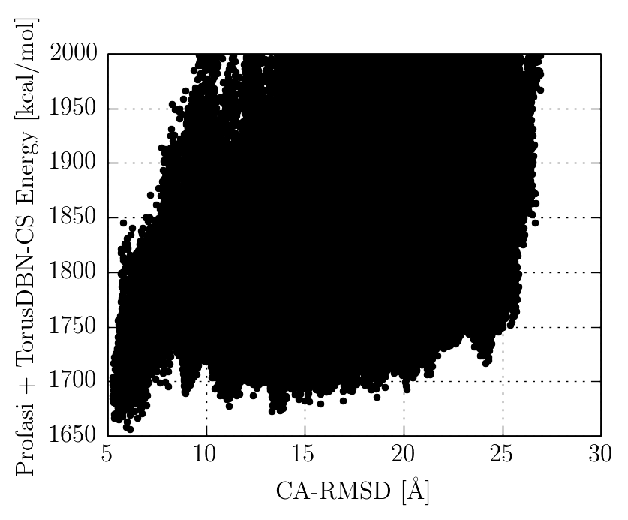
\includegraphics[width=0.4\textwidth]{figures/rhodopsin_figures/folding_data.pdf}}
    }\quad
    \subfloat[Energy-scoring during refinement stage.]{
        {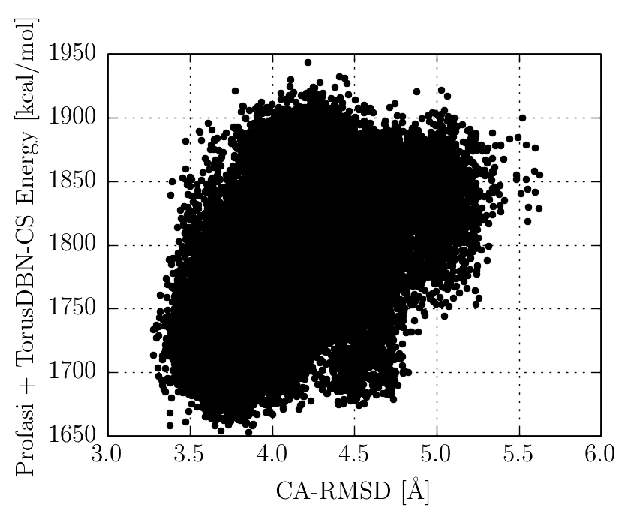
\includegraphics[width=0.4\textwidth]{figures/rhodopsin_figures/refinement_data.pdf}}
    }\\
%    \subfloat[Bottom view of folding stage lowest energy sample (blue).]{
%        {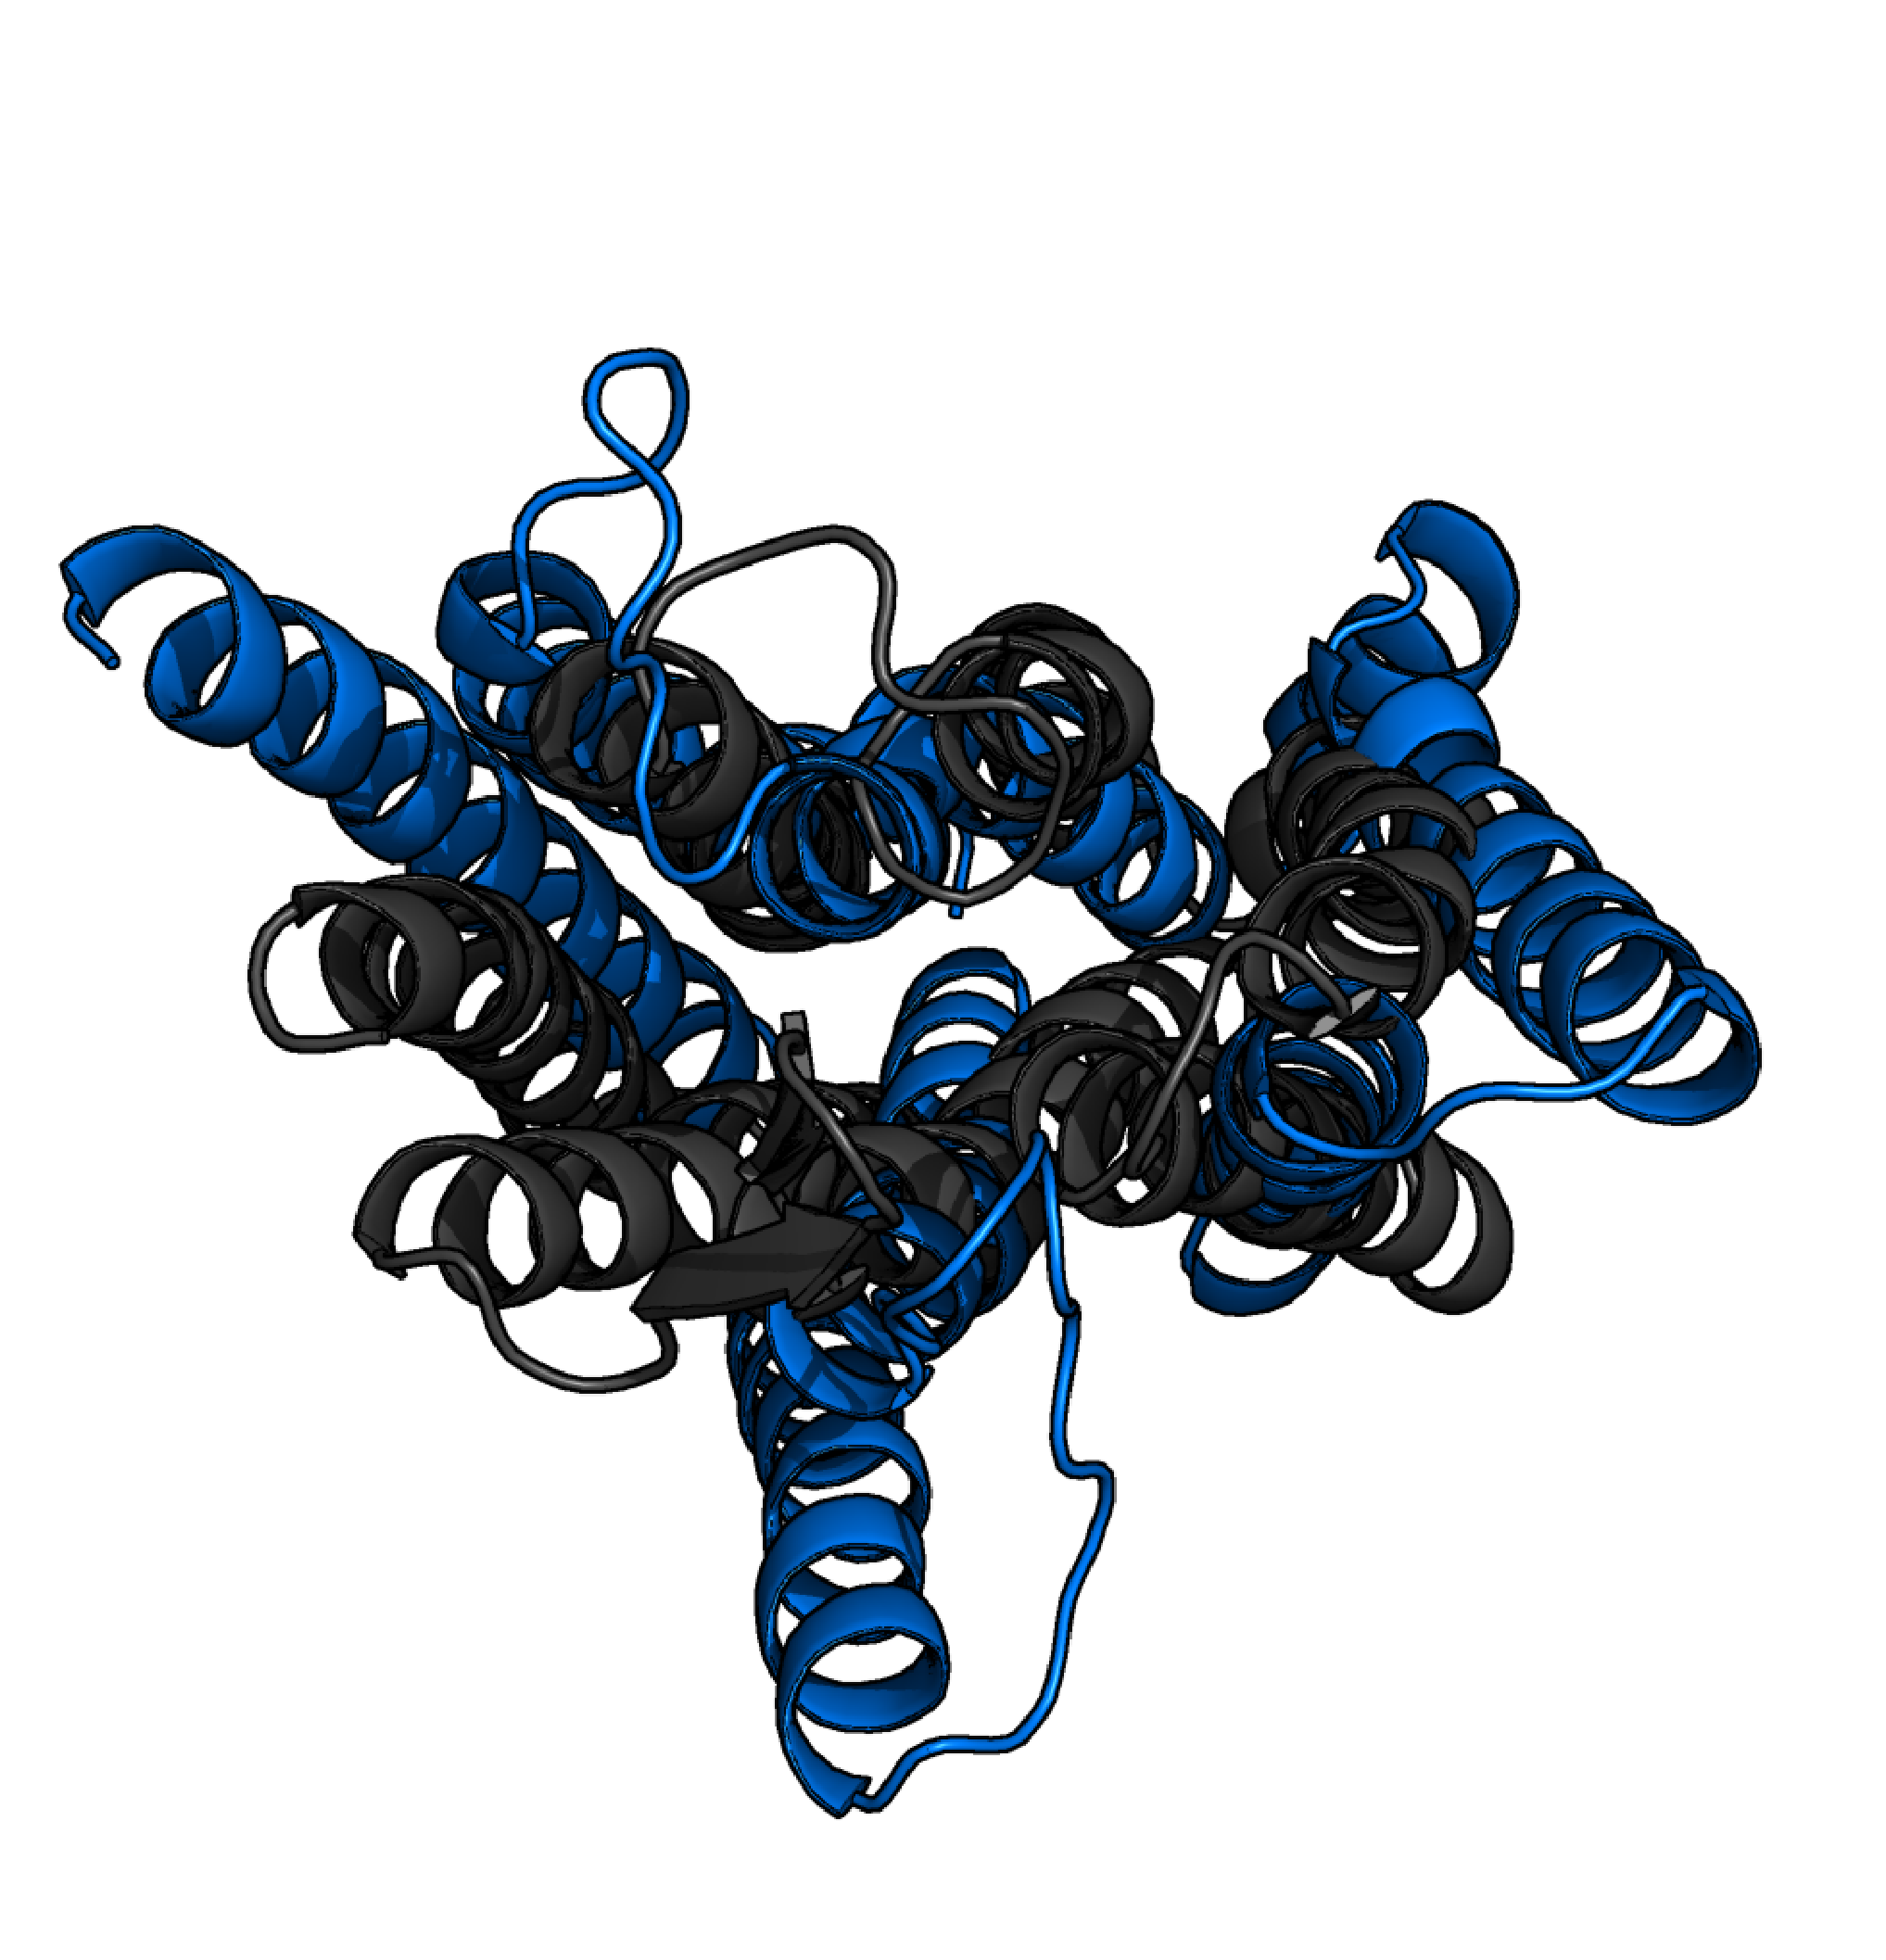
\includegraphics[width=0.4\textwidth]{figures/rhodopsin_figures/folding_bottom.pdf}}
%    }\quad
%    \subfloat[Bottom view of refinement stage lowest energy sample (red).]{
%        {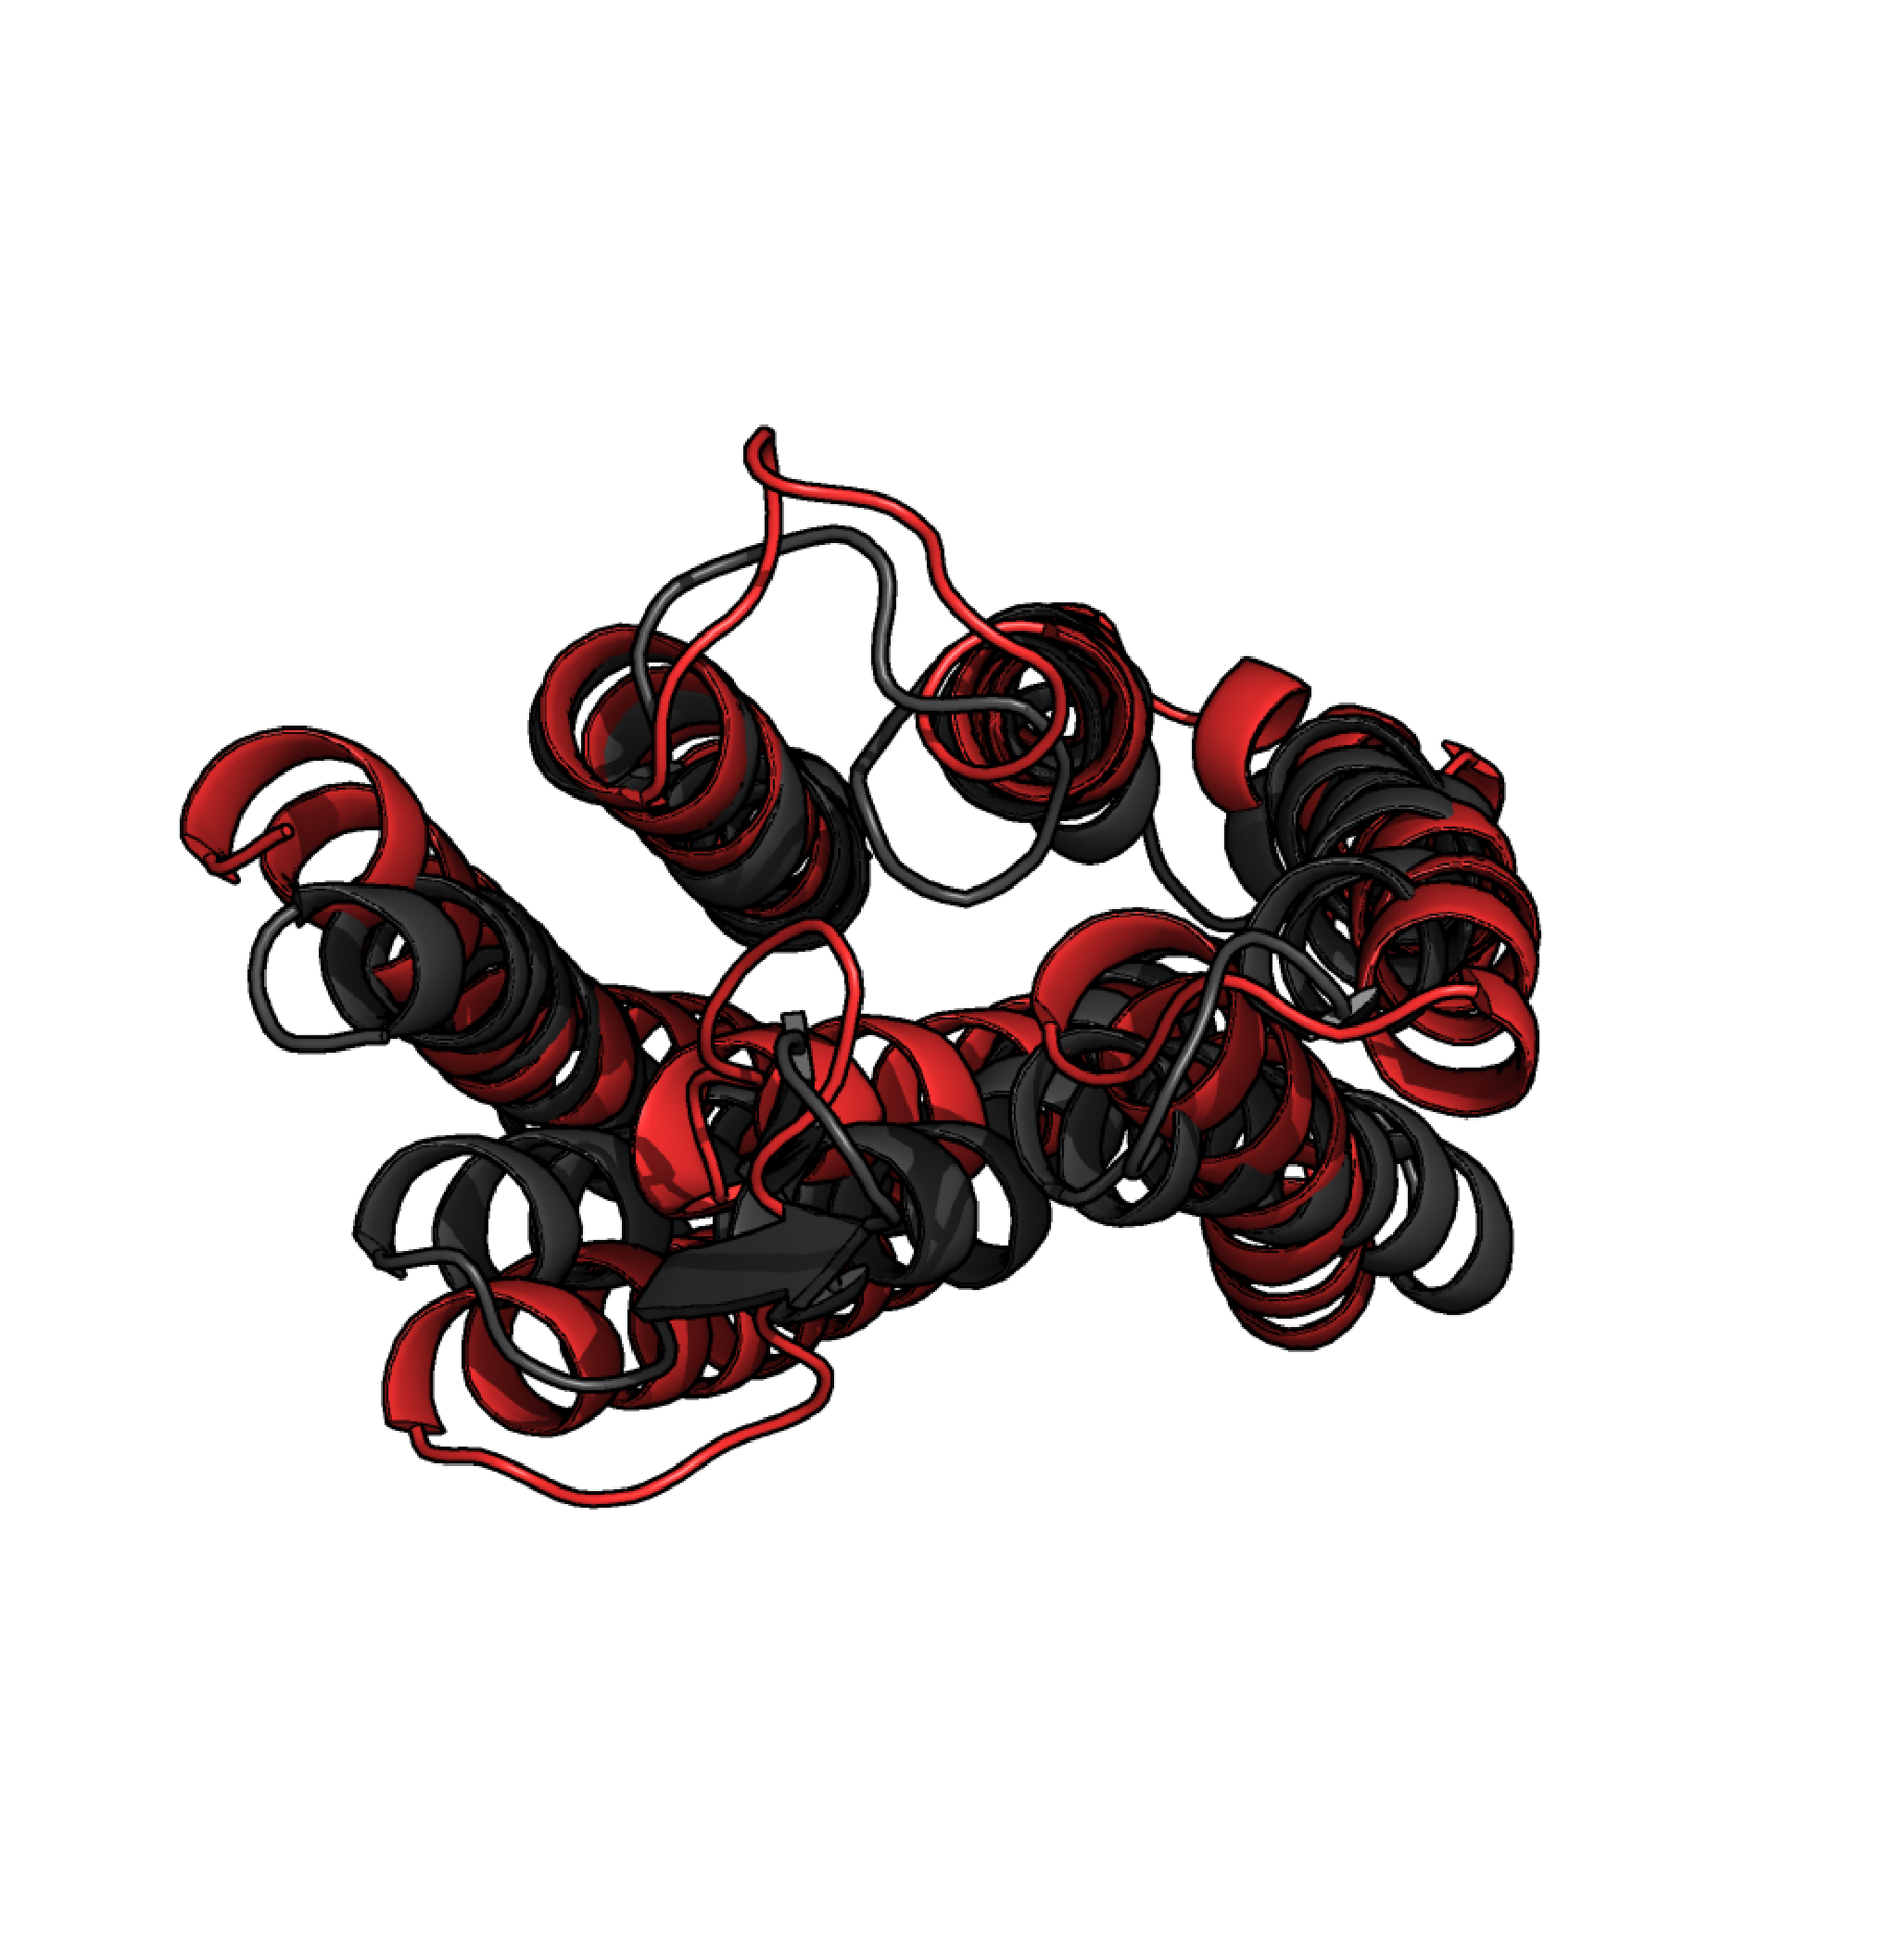
\includegraphics[width=0.4\textwidth]{figures/rhodopsin_figures/refinement_bottom.pdf}}
%    }\\
    \subfloat[Folding stage lowest energy sample (blue). 7.8 \AA~CA-RMSD.]{
        {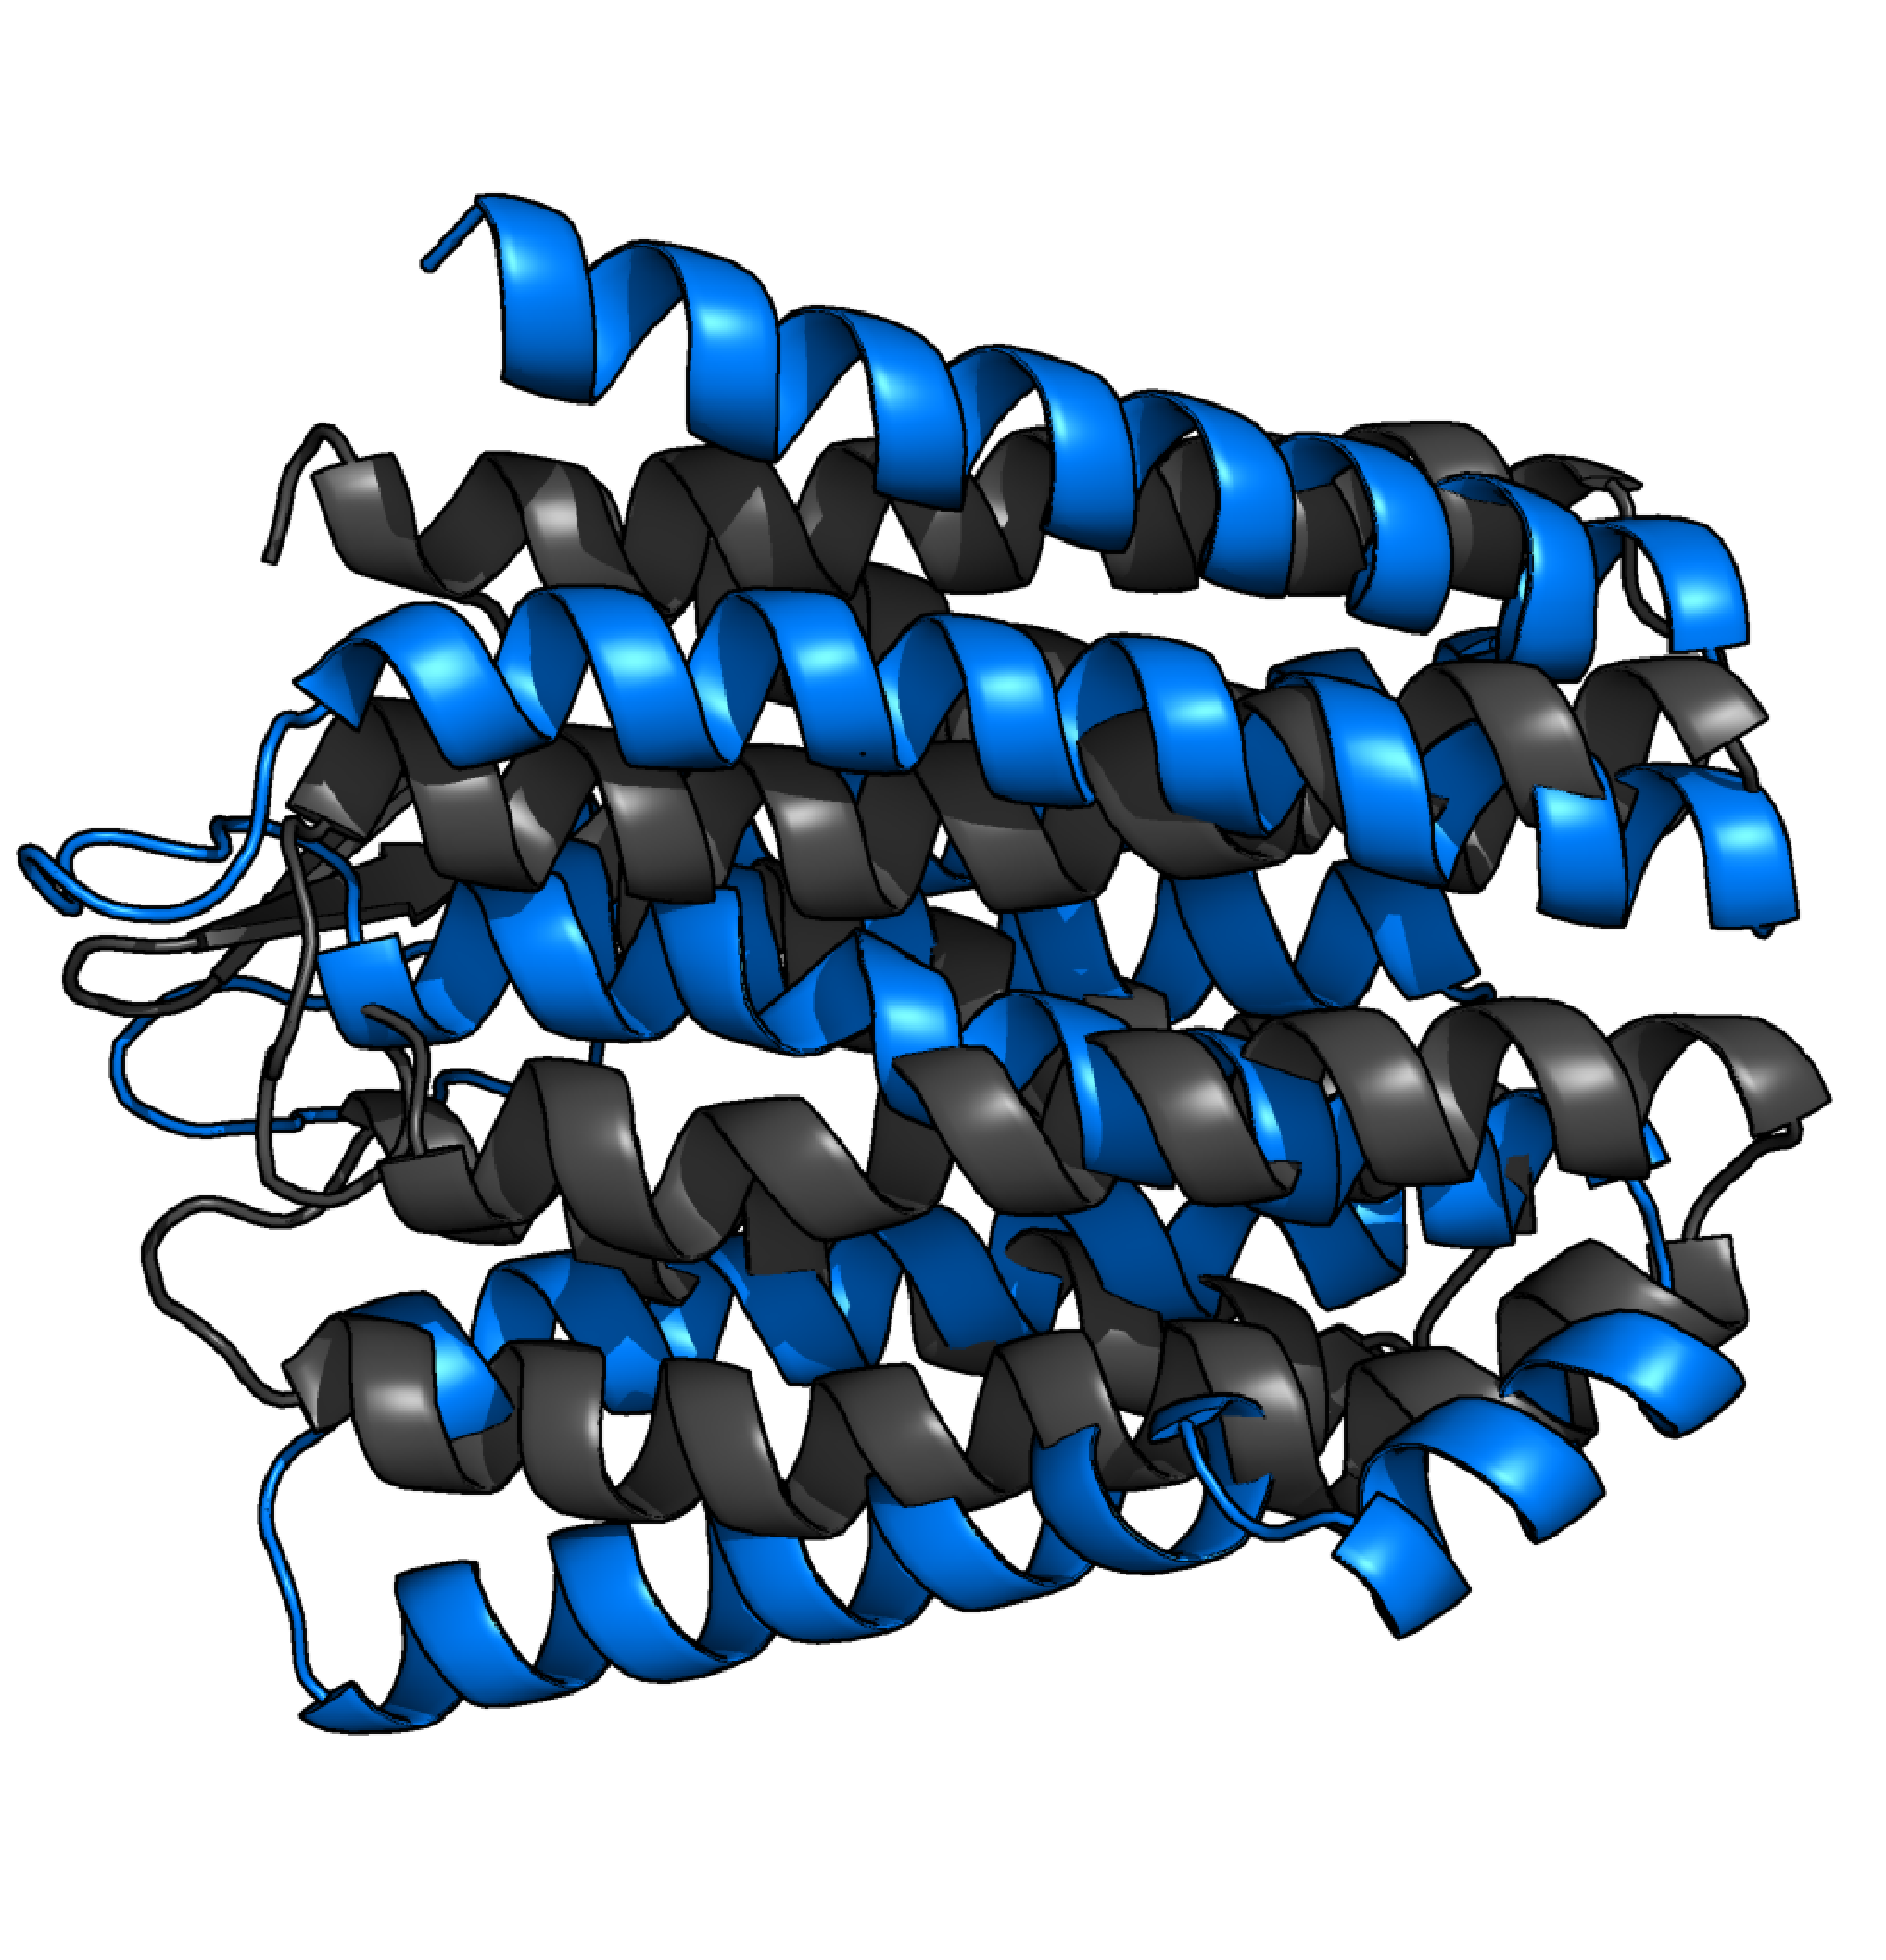
\includegraphics[width=0.4\textwidth]{figures/rhodopsin_figures/folding.pdf}}
    }\quad
    \subfloat[Refinement stage lowest energy sample (blue). 2.5 \AA~CA-RMSD. ]{
        {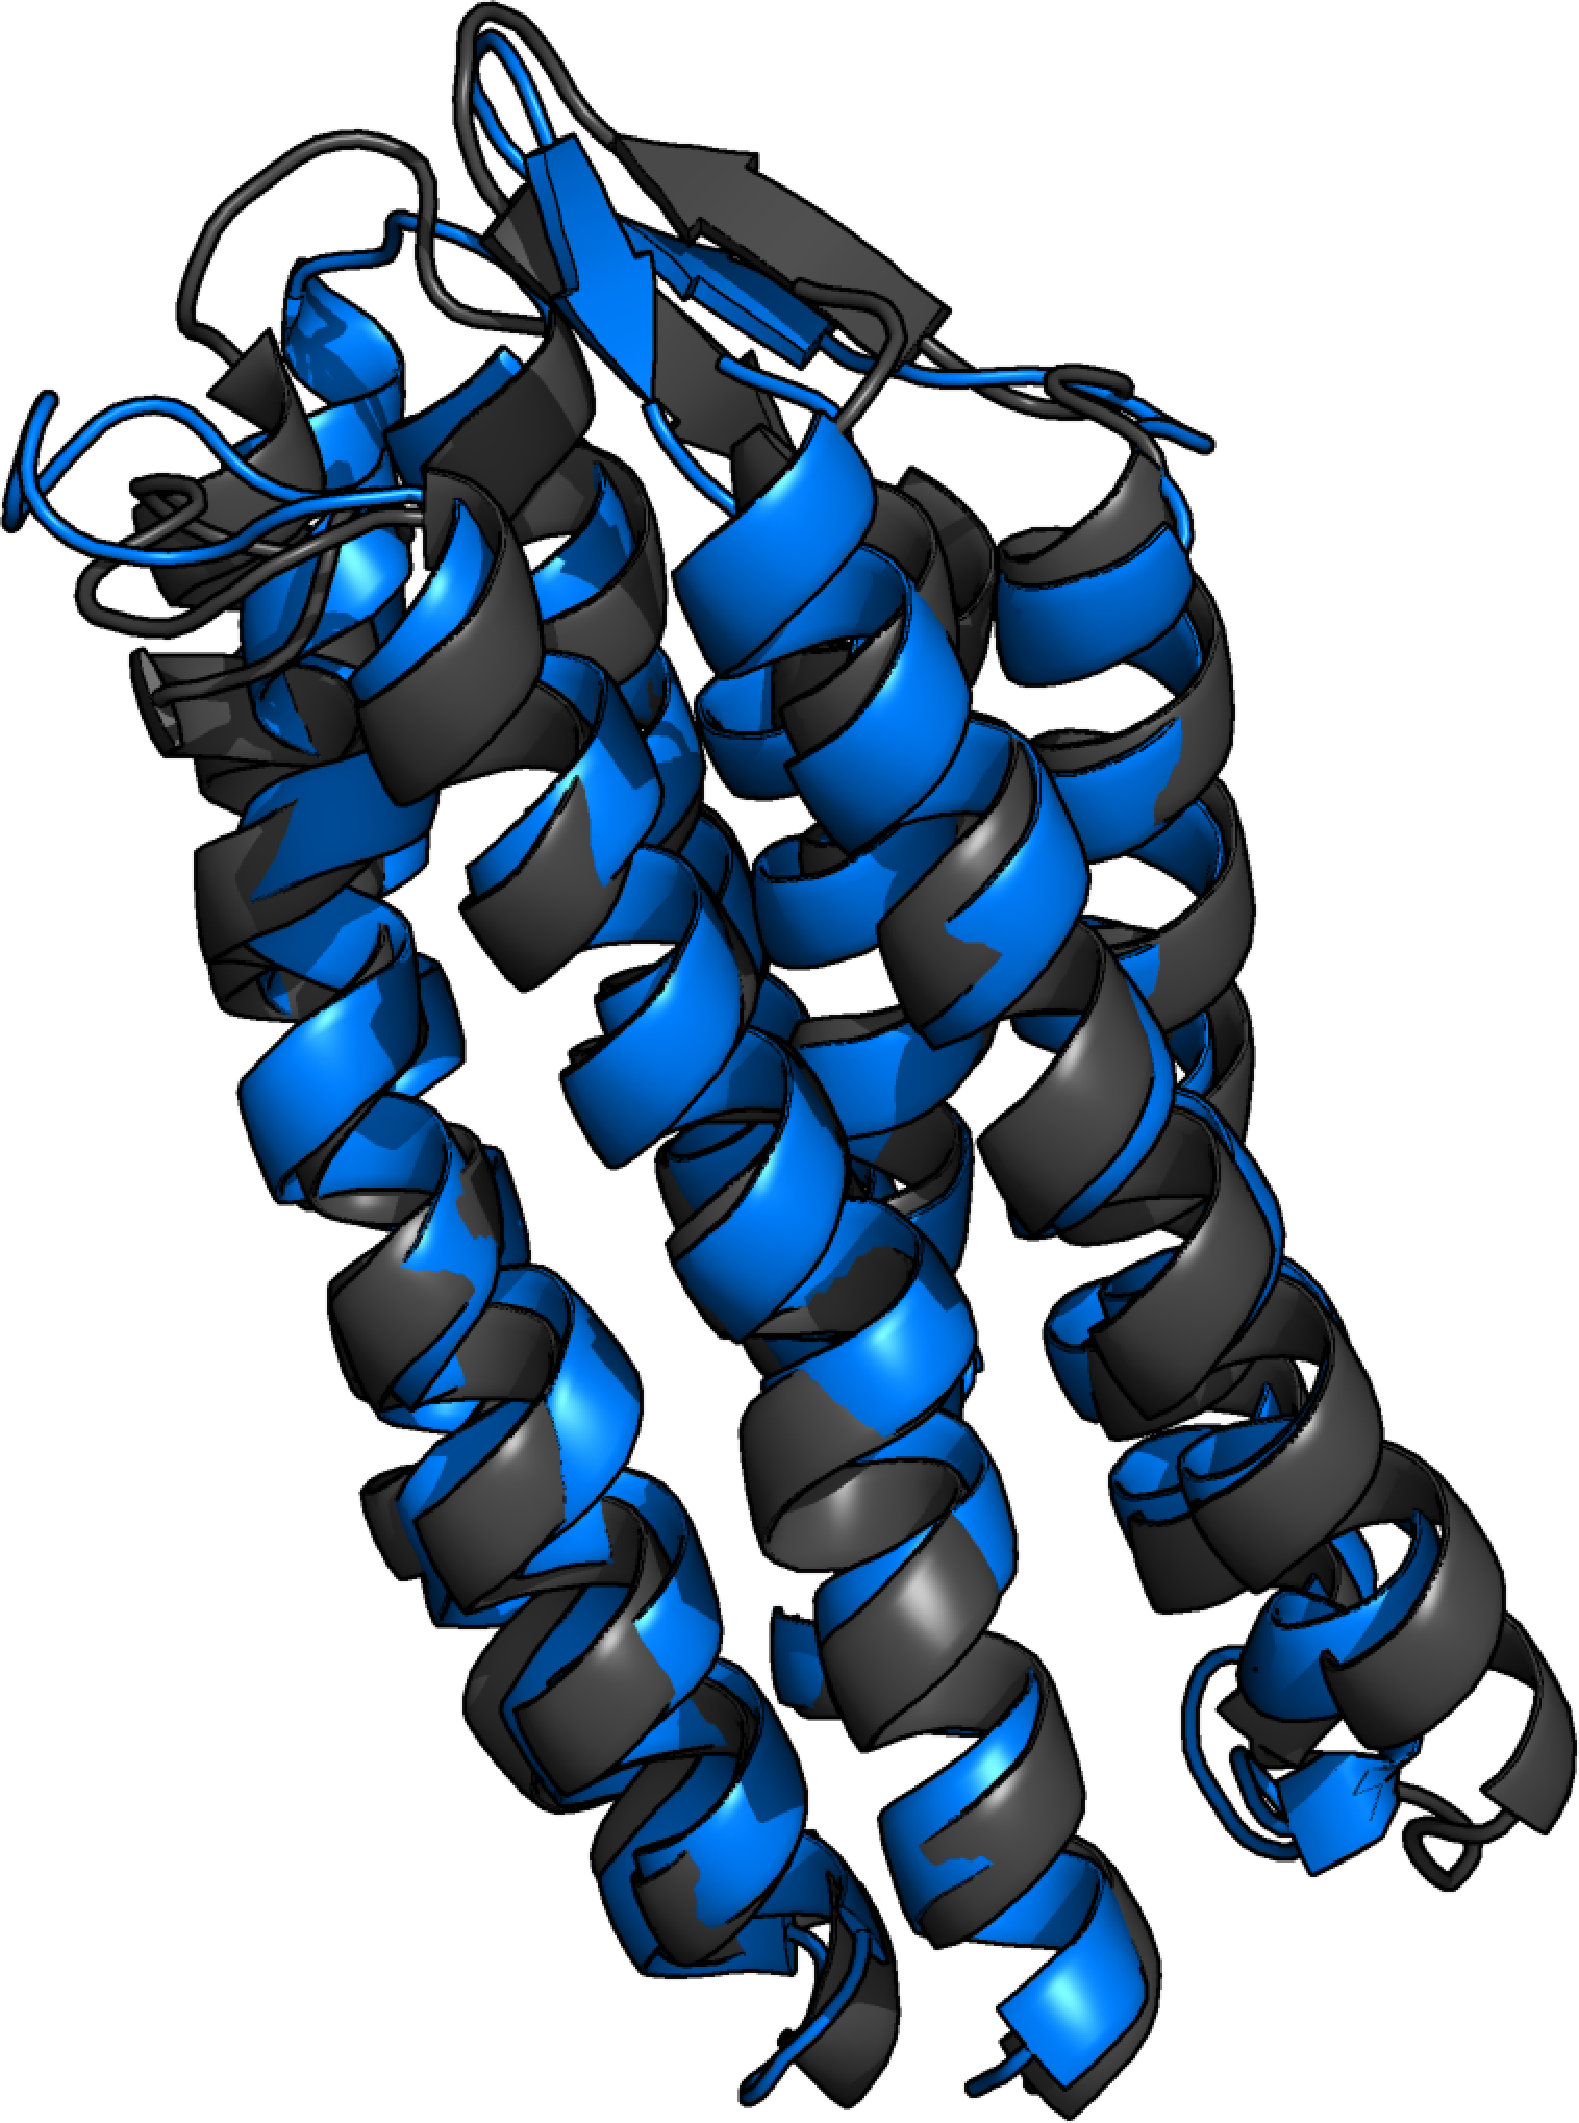
\includegraphics[width=0.4\textwidth]{figures/rhodopsin_figures/lowest_e.pdf}}
    }\\
    \caption{(a) displays the energy scoring during the folding stage of Rhodopsin, and (b) the same statistics during the refinement stage. (c) displays the lowest energy structure after the folding stage, and (d) the lowest energy structure after the refinement stage.}
    \label{fig:rhodopsin}%
\end{figure}


\begin{figure}%
    \centering
    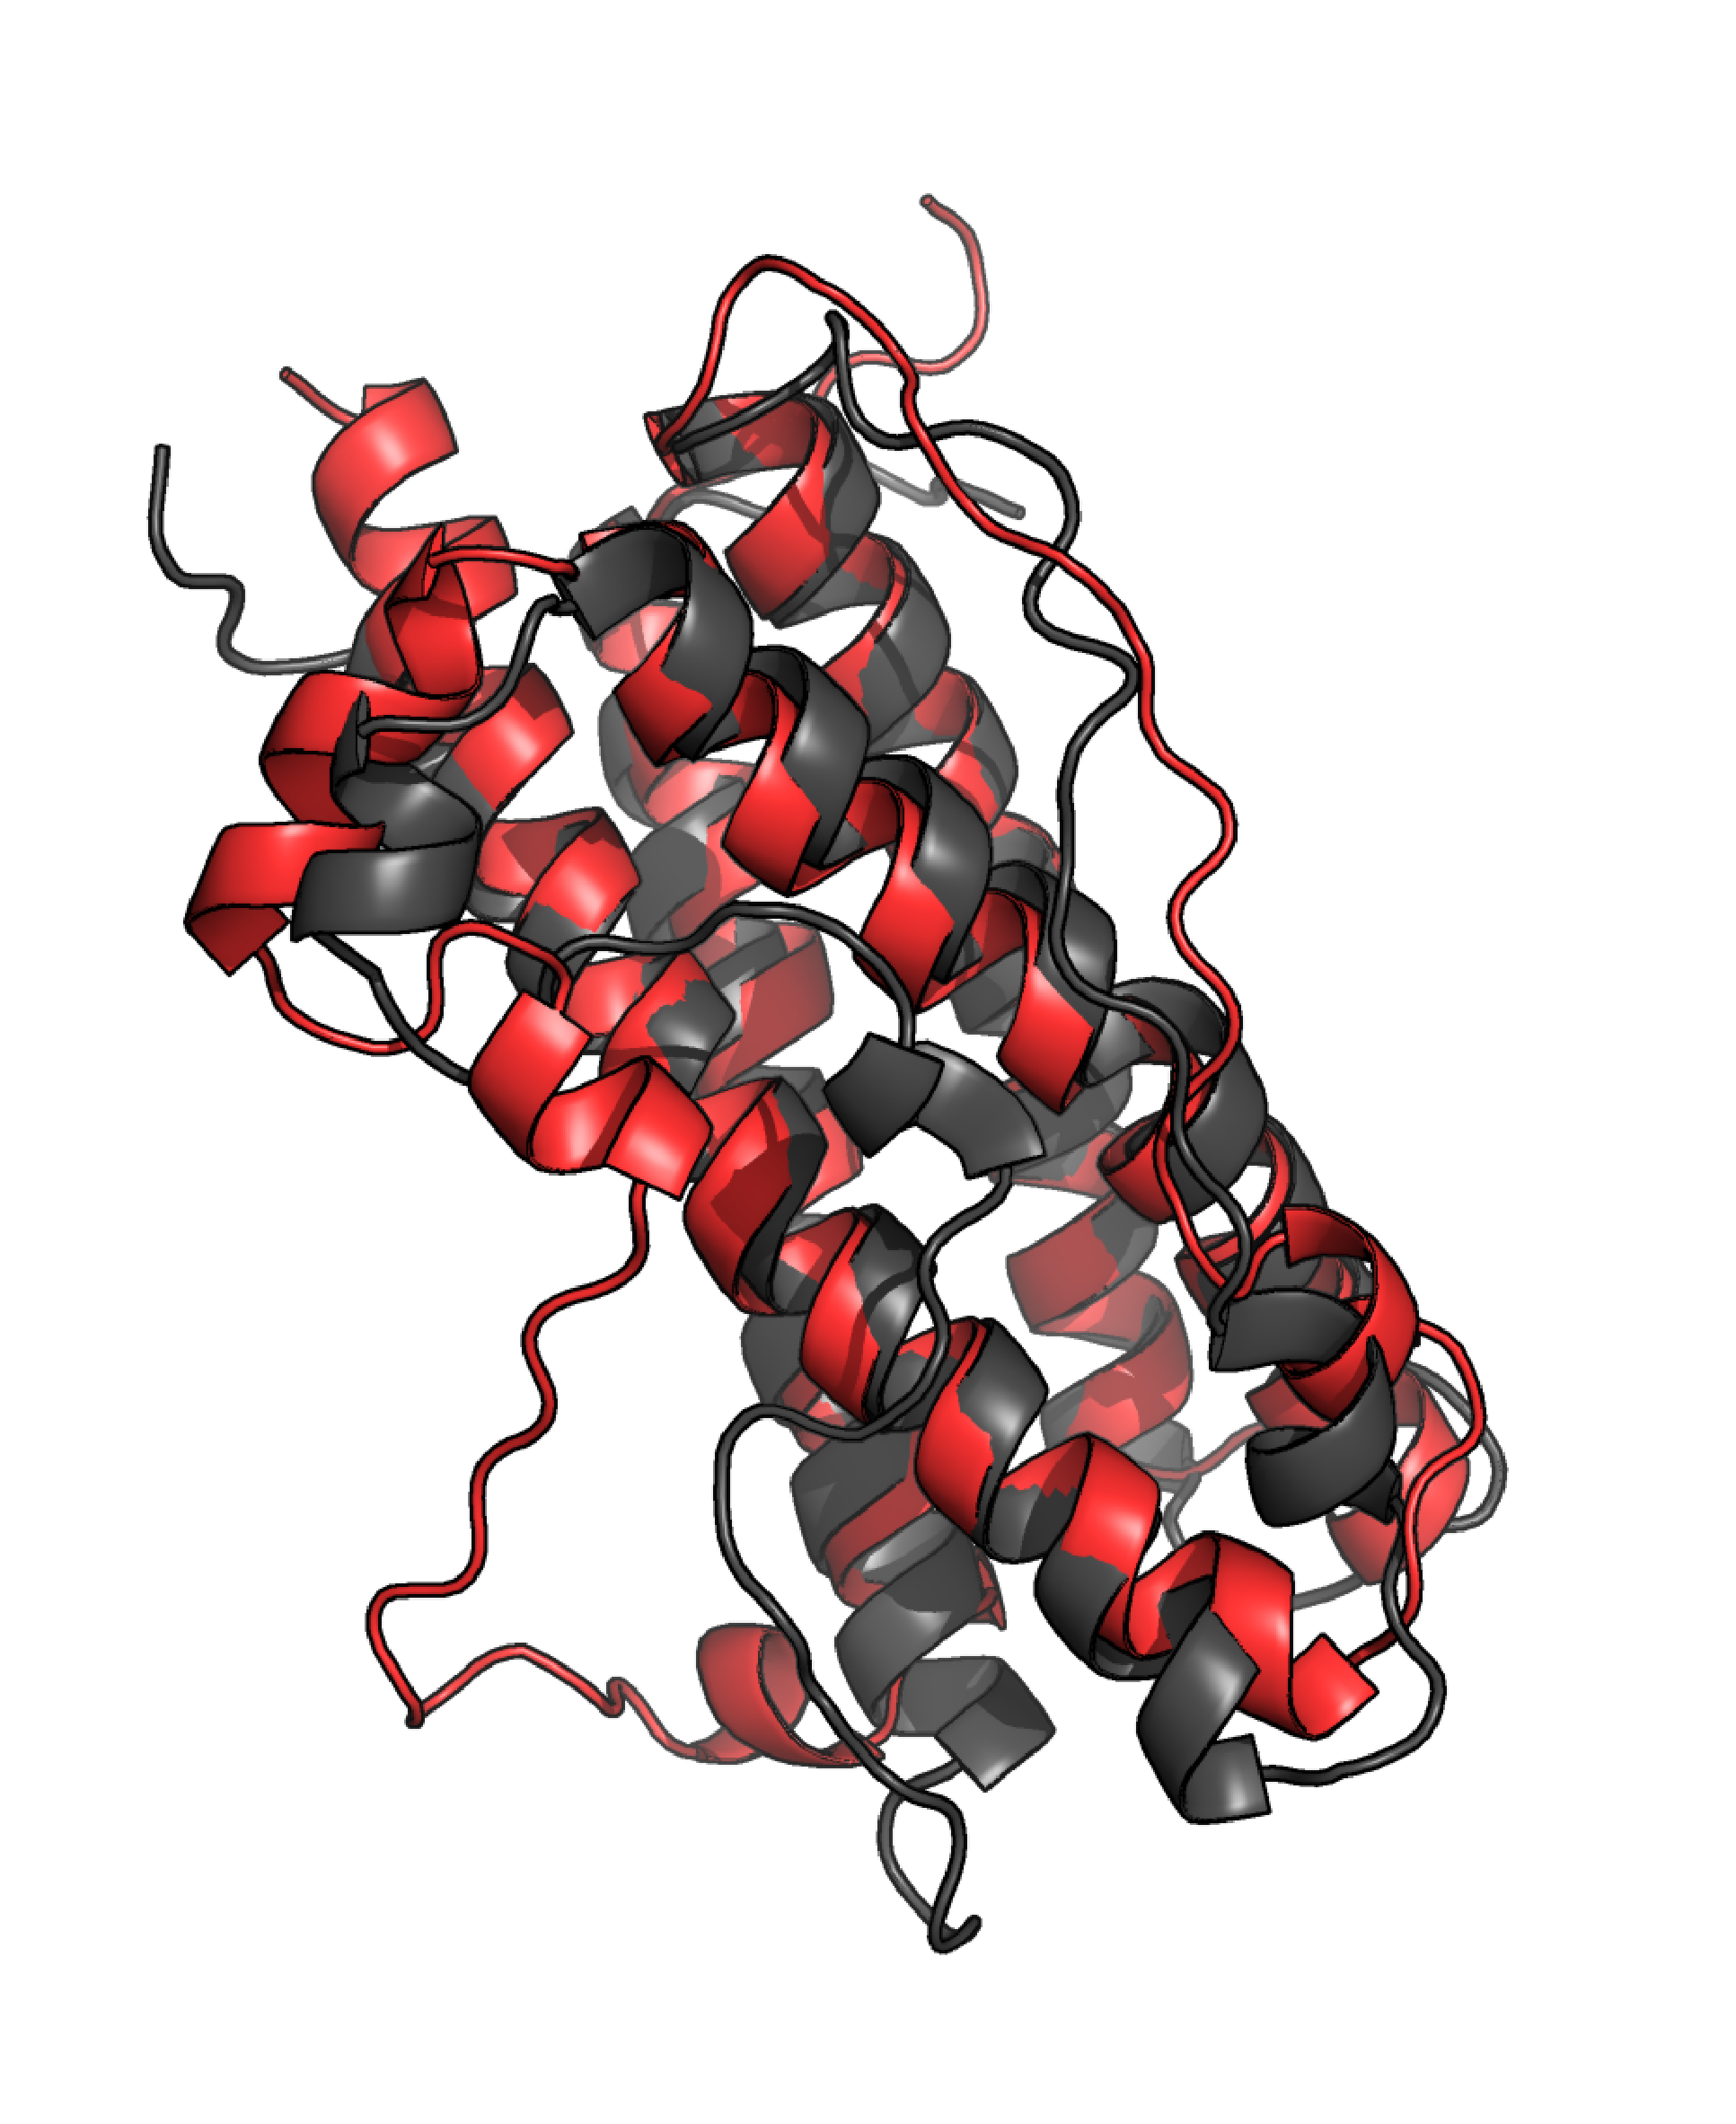
\includegraphics[width=\textwidth]{figures/prolactin_lowest_e.pdf}
    \caption{The lowest energy sample (red) for Prolactin after refinement. Note the flexible part which is not in agreement with the experimental X-ray structure (grey).}
    \label{fig:prolactin}%
\end{figure}




\clearpage


\section{Evolutionary distance constraints}

\begin{figure}%
    \centering
    \subfloat[Lowest RMSD sample]{
        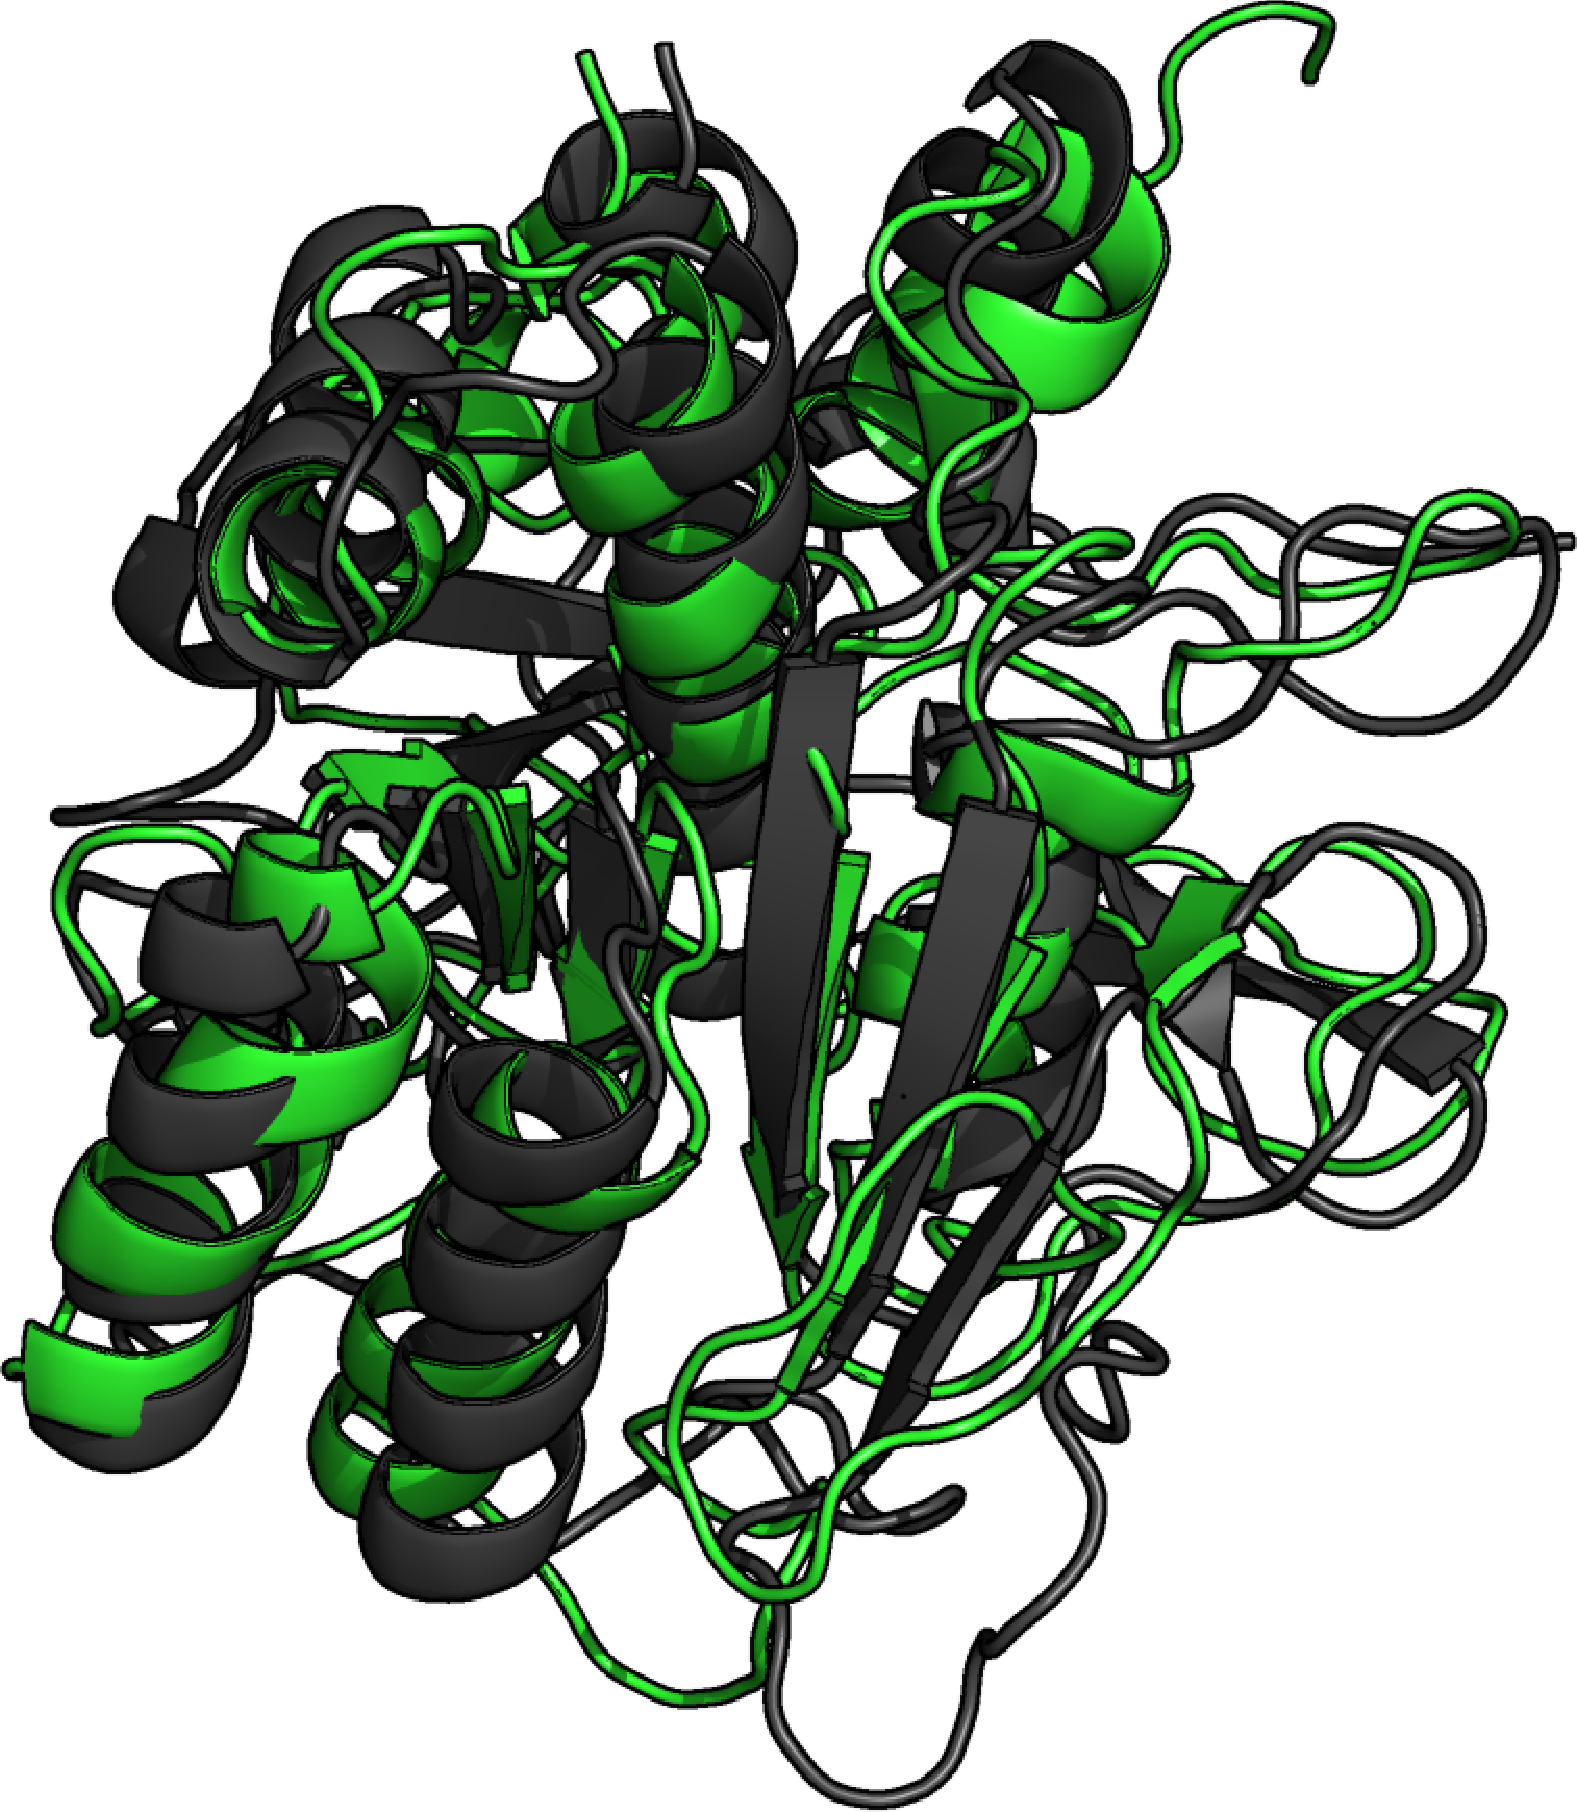
\includegraphics[width=0.40\textwidth]{figures/savinase_fold/savinase_lowest_e.pdf}
        %{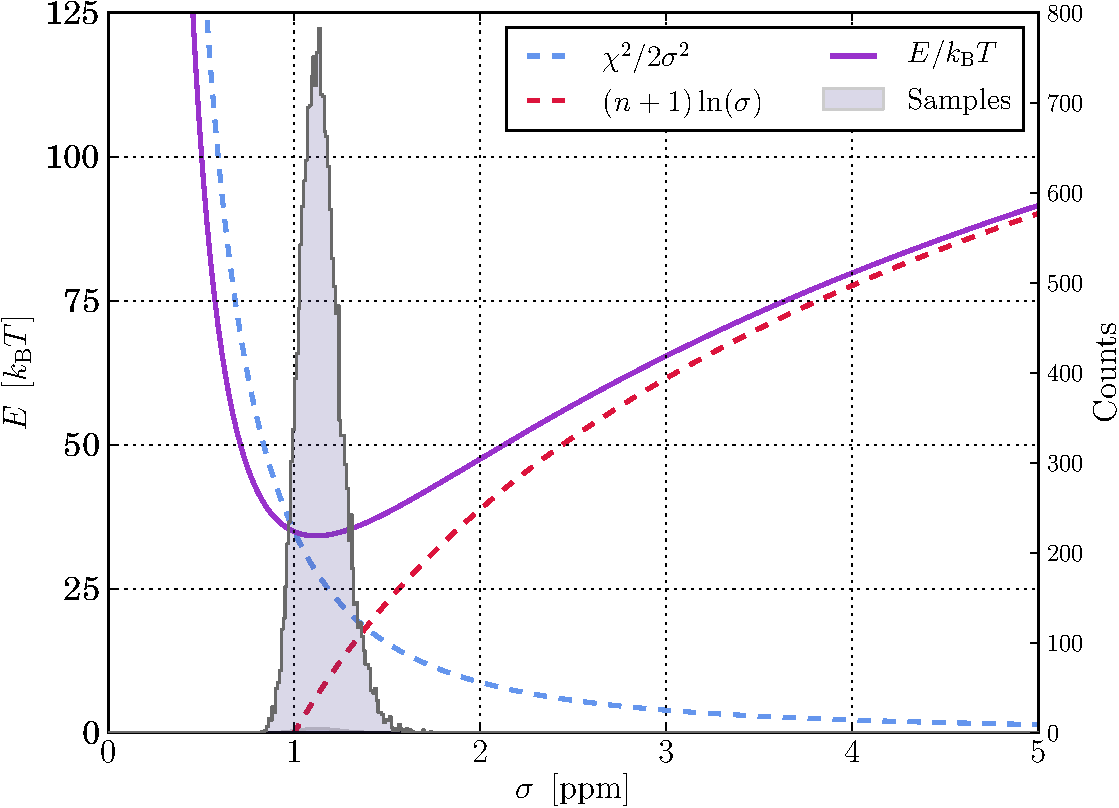
\includegraphics[width=0.42\textwidth]{sigma_prior.pdf} }
    }
    \subfloat[Lowest energy sample]{
        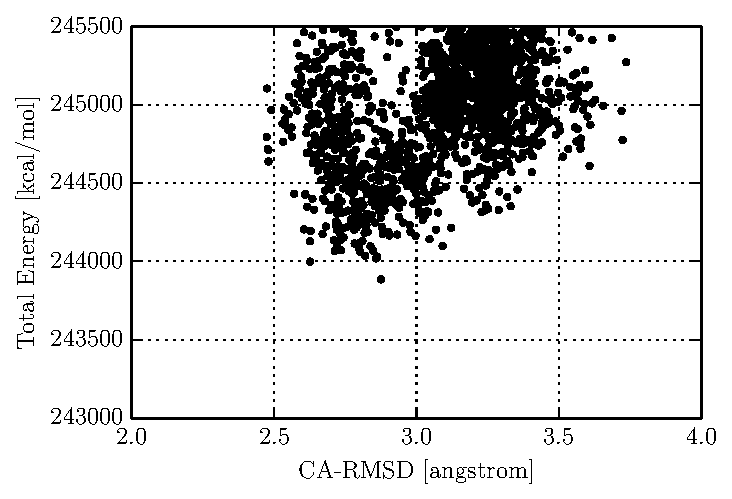
\includegraphics[width=0.60\textwidth]{figures/savinase_fold/savinase_refinement.pdf}
    }
    \caption{Refinement stage of the savinase simulation. The lowest energy sample has a CA-RMSD of 2.9 \AA. }
    \label{fig:savinase_fold}%
\end{figure}


As discussed previously, it is increasingly difficult to obtain sufficient distance restraints as the size of the protein increases.
A recently developed methodology uses sequence analysis to infer residue contacts in 3D space \cite{evfold}.
In brief, the method works by identifying sequence co-variation, which retains favorable contacts between residues.
This way, pair of residues which are probable to be close in 3D space can be identified.
The procedure is briefly summarized in Fig.~\ref{fig:evo_constraint}, and is implemented in the EVfold program.

In this proof-of-concept study, 270 contacts were obtained a multiple-sequence alignment using the EVfold program (Wouter Boomsma, personal communications) for the 269 residue protein Savinase.
The restraints were simply treated as NOE restraints using old NOE code mentioned in the previous section.
A similar simulation to that which folded Rhodopsin was adopted. 
In terms of computational resources, these were increased to 100 threads and $75 \times 10^6$ iterations, compared to only 72 threads and $50 \times 10^6$ iterations for the Rhodopsin simulation.
One thread identified a native-like structure.

The folding simulation yielded a lowest energy structure around 7.5 \AA~CA-RMSD from native. A further refinement with the new NOE code from this structure, yielded a lowest RMSD structure at 2.9 \AA~CA-RMSD from the X-ray structure.
The structure and an energy/RMSD plot for the refinement is shown in Fig.~\ref{fig:savinase_fold}.

\begin{figure}
    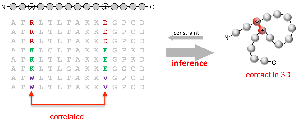
\includegraphics[width=0.85\textwidth]{figures/evo_constraint.pdf}
    \caption{Evolutionary constraints}
    \label{fig:evo_constraint}
\end{figure}

% \begin{figure}
%     \centering
%     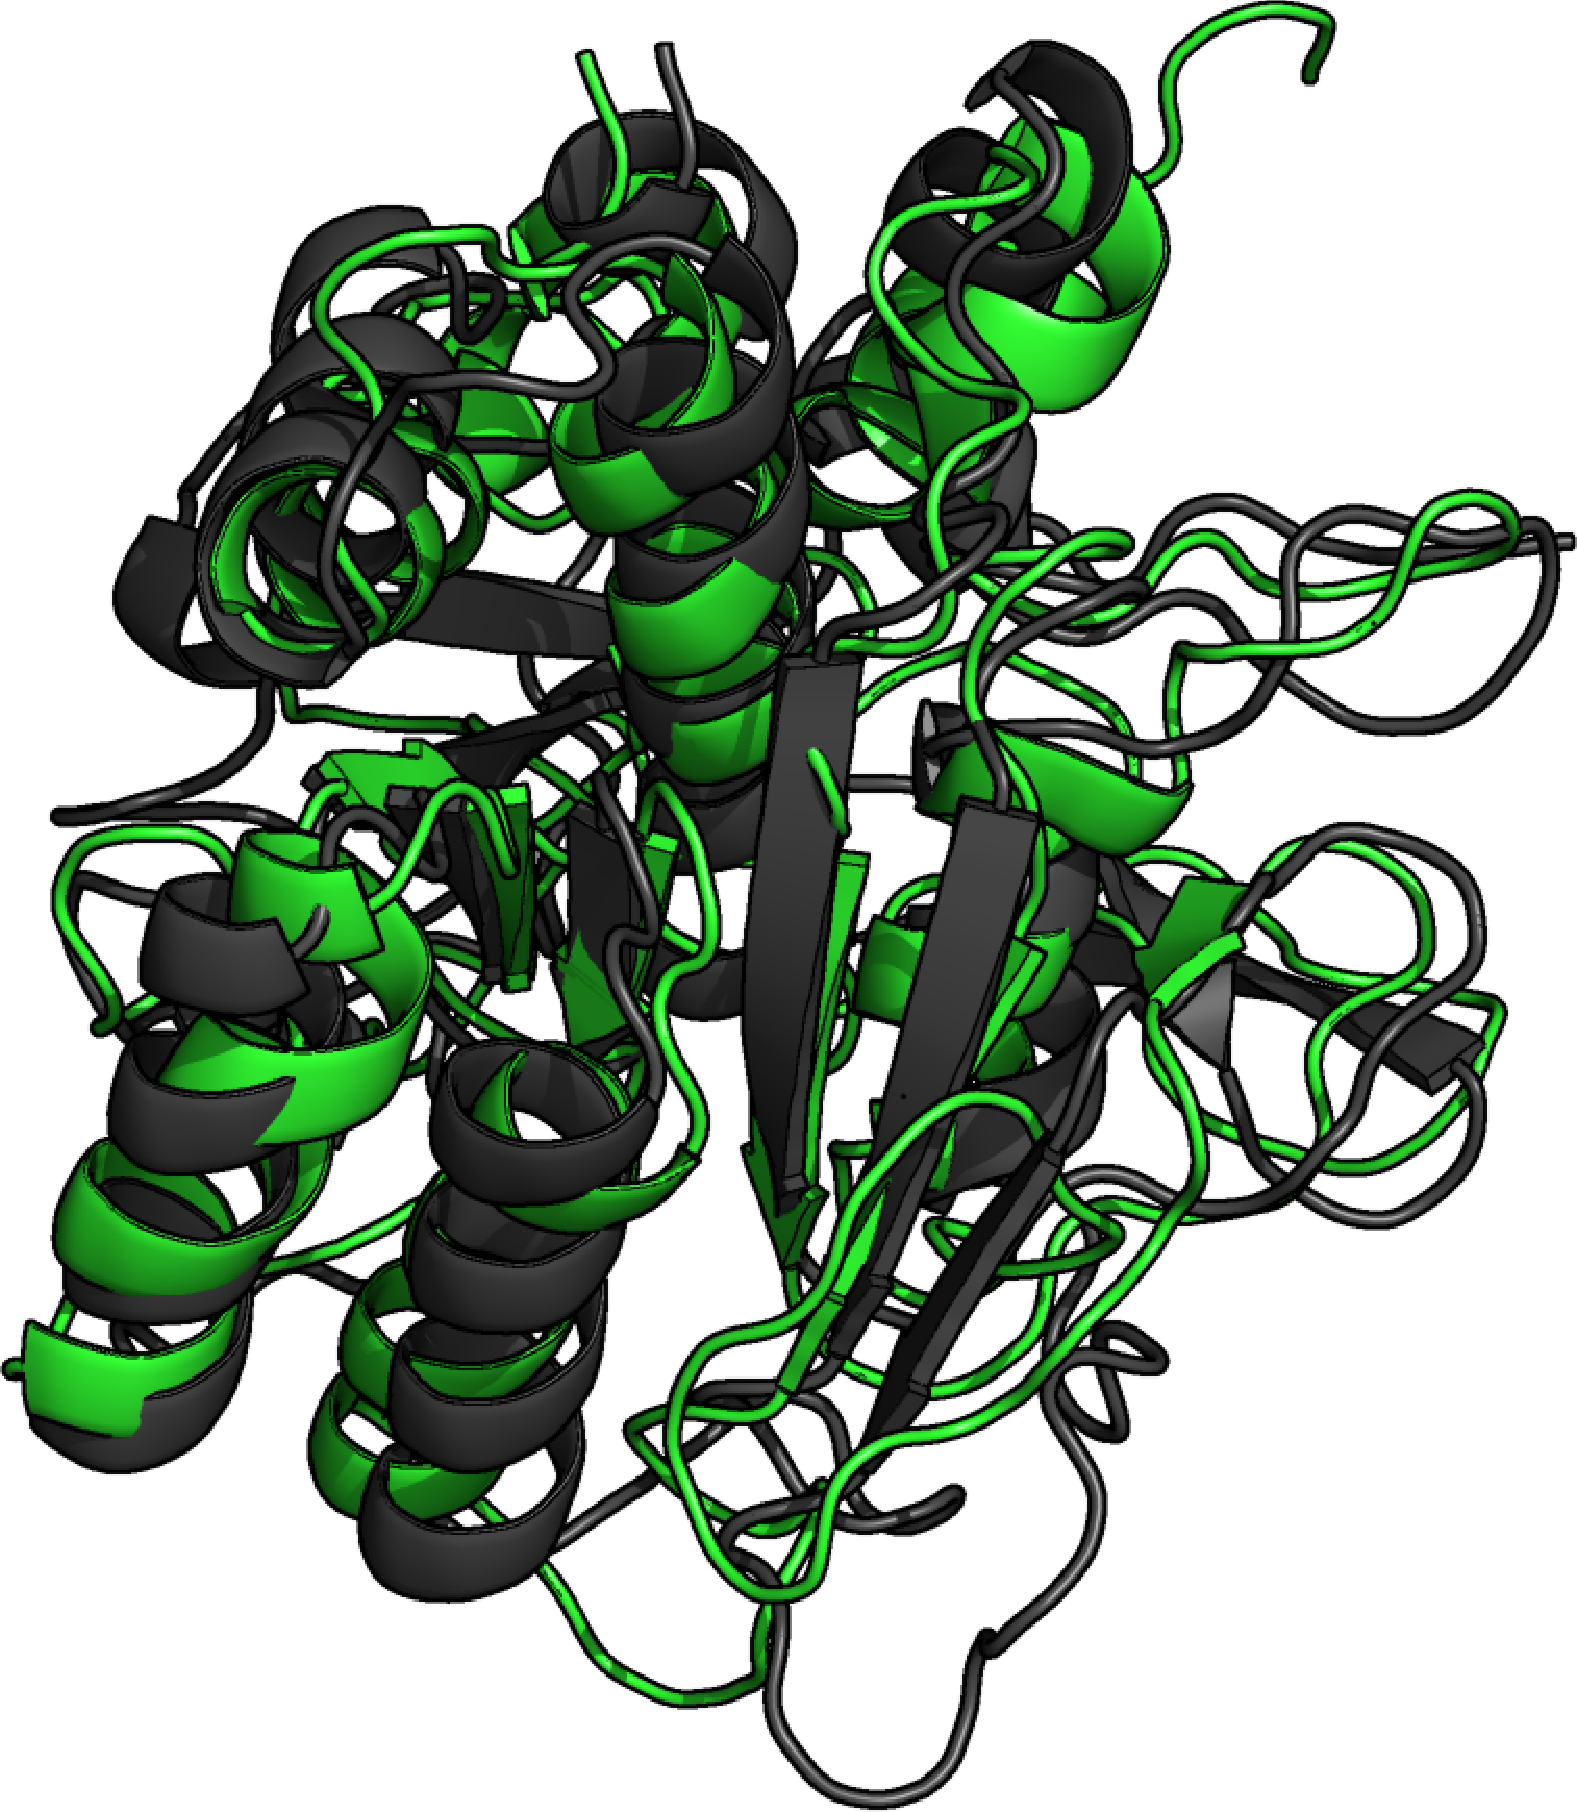
\includegraphics[width=0.60\textwidth]{figures/savinase_fold/savinase_lowest_e.pdf}
%     \caption{The lowest energy structure of Savinase after the refinement (green) and the 
%              1SVN crystal structure (grey). The CA-RMSD is 2.9 \AA.}
%     \label{fig:savinase_align}
% \end{figure}




% 
% \begin{figure}
%     \centering
%     \caption{Savinase folded}
%     \label{fig:savinase_align}
% \end{figure}
% 

